% Compile with XeLaTeX !!
\documentclass[12pt,a4paper]{article}

% -------------------------------------------------
% Fonts & Greek language via polyglossia
% -------------------------------------------------
\usepackage{fontspec}
\usepackage{polyglossia}

\setmainlanguage{greek}
\setotherlanguage{english}

\setmainfont{Times New Roman}
\setsansfont{Arial}
\setmonofont{Courier New}

% -------------------------------------------------
% Math & Formatting
% -------------------------------------------------
\usepackage{amsmath, amssymb, amsfonts}
\usepackage{geometry}
\usepackage{float}
\usepackage{hyperref}
\usepackage{caption}
\usepackage{graphicx}
\usepackage{multirow}
\usepackage{multirow}

\geometry{margin=2.5cm}

\title{\textbf{Τεχνικές Βελτιστοποίησης}\\
	\large 2η Εργαστηριακή Άσκηση}
\author{Πελοπίδας-Νικόλαος Τσιούντσιουρας \\ ΑΕΜ: 11085}
\date{\today}

\begin{document}
	
	\maketitle
	\tableofcontents
	\newpage
	
	% ======================================================
	% 1. Εισαγωγή
	% ======================================================
	\section{Εισαγωγή}
	
	Στην παρούσα εργασία εξετάζεται το πρόβλημα ελαχιστοποίησης μιας μη γραμμικής συνάρτησης δύο μεταβλητών χωρίς περιορισμούς:
	
	\[
	f(x,y) = x^{3} e^{-(x^{2} + y^{2})}.
	\]
	
	Η συνάρτηση παρουσιάζει έντονη μη γραμμικότητα, περιοχές απότομης μεταβολής και πιθανή ύπαρξη πολλών τοπικών ακροτάτων. Αντικείμενο της εργασίας είναι η μελέτη τριών κλασικών αλγορίθμων εύρεσης ελαχίστου:
	
	\begin{itemize}
		\item \textbf{Μέθοδος Μέγιστης Καθόδου (Steepest Decent)},
		\item \textbf{Μέθοδος Newton},
		\item \textbf{Μέθοδος Levenberg–Marquardt}.
	\end{itemize}
	
	Και οι τρεις μέθοδοι βασίζονται σε επαναληπτική διαδικασία εύρεσης νέων σημείων:
	
	\[
	x_{k+1} = x_k + \gamma_k d_k,
	\]
	
	όπου \(d_k\) είναι η κατεύθυνση αναζήτησης και \(\gamma_k\) το βήμα.  
	Οι μέθοδοι εφαρμόζονται για τρία διαφορετικά αρχικά σημεία:
	
	\[
	(x_0,y_0) \in \{(0,0), (-1,-1), (1,1)\},
	\]
	
	και η ανάλυση επικεντρώνεται:
	
	\begin{itemize}
		\item στη σύγκλιση,
		\item στον αριθμό επαναλήψεων,
		\item στην επίδραση της επιλογής του βήματος,
		\item στην εξάρτηση από το αρχικό σημείο,
		\item στη σύγκριση των μεθόδων.
	\end{itemize}
	
	\newpage
	
	% ======================================================
	% 2. Θεωρία
	% ======================================================
	\section{Θεωρία}
	
	Η συνάρτηση \(f(x,y) = x^{3} e^{-(x^{2}+y^{2})}\) είναι συνεχώς διαφορίσιμη και επιτρέπει τον υπολογισμό κλίσης και Hessian.
	
	\subsection{Κλίση και Hessian}
	
	Η κλίση δίνεται από:
	
	\[
	\nabla f(x,y) =
	\begin{pmatrix}
		3x^{2}e^{-(x^{2}+y^{2})} - 2x^{4}e^{-(x^{2}+y^{2})} \\
		-2x^{3}y\,e^{-(x^{2}+y^{2})}
	\end{pmatrix}.
	\]
	
	Το Hessian αποτελείται από τις δεύτερες μερικές παράγωγες και χρησιμοποιείται στη μέθοδο Newton και Levenberg–Marquardt.
	
	\subsection{Μέθοδος Μέγιστης Καθόδου}
	
	Η μέθοδος \textbf{Steepest Descent} αποτελεί την πιο βασική τεχνική κατεύθυνσης καθόδου και βασίζεται στην ιδέα ότι η κλίση της συνάρτησης δείχνει πάντοτε την κατεύθυνση μέγιστης αύξησης· συνεπώς, η αρνητική κλίση αποτελεί φυσική επιλογή για την αναζήτηση ελαχίστου. Παρότι η μέθοδος είναι απλή, σταθερή και με χαμηλό υπολογιστικό κόστος σε κάθε επανάληψη, χαρακτηρίζεται από αργό ρυθμό σύγκλισης, ειδικά σε περιοχές όπου οι ισοϋψείς καμπύλες της συνάρτησης έχουν έντονη ανισοτροπία, οδηγώντας σε μια χαρακτηριστική «ζιγκ–ζαγκ» πορεία προς το ελάχιστο. Η επιλογή του βήματος γινόμενη μέσω κατάλληλου line search (minimize ή Armijo) βελτιώνει σημαντικά την αποδοτικότητα, μειώνοντας δραστικά τον αριθμό επαναλήψεων.
	Αναλυτικά ο αλγόριθμος:
	\begin{itemize}
		\item Ορίστε $\epsilon>0$ τη σταθερά τερματισμού. Επιλέξτε το αρχικό σημείο $x_1$ και θέστε $k=1$.
		\item Αν $|\nabla f(x_k)|<\epsilon$ ο αλγόριθμος τερματίζει. Διαφορετικά, θέστε $d_k=-\nabla f(x_k)$ και ορίστε το $\gamma_k$ ανάλογα με τον κανόνα που επιλέγεται το $\gamma$ (σταθερό, minimize, armijo). Θέστε $x_{k+1}=x_k-\gamma_k\nabla f(x_k)$, $k=k+1$ και επαναλάβετε.
	\end{itemize}
	
	\subsection{Μέθοδος Newton}
	
	Η \textbf{μέθοδος Newton} αποτελεί μια από τις ταχύτερες τεχνικές βελτιστοποίησης όταν η συνάρτηση είναι ομαλή και το Hessian θετικά ορισμένο κοντά στο ελάχιστο, προσφέροντας τετραγωνική σύγκλιση. Εκμεταλλεύεται πληροφορία δεύτερης τάξης ώστε να προσαρμόζει τη διεύθυνση αναζήτησης βάσει της τοπικής καμπυλότητας, γεγονός που της επιτρέπει να εντοπίζει γρήγορα την περιοχή ελαχιστοποίησης. Ωστόσο, η απόδοσή της εξαρτάται κρίσιμα από το αρχικό σημείο και τη μορφή του Hessian: εάν η συνάρτηση διαθέτει σέλες, μη θετικά ορισμένο Hessian ή περιοχές με έντονη ανισοτροπία, η μέθοδος μπορεί να αποτύχει να κατέβει προς το ελάχιστο ή να παρουσιάσει πολύ αργή πρόοδο. Η εφαρμογή line search βελτιώνει τη σταθερότητα, αλλά δεν εξαλείφει πλήρως τα προβλήματα από λανθασμένες κατευθύνσεις Newton. Παρά τους περιορισμούς της, παραμένει η πιο αποτελεσματική μέθοδος όταν το αρχικό σημείο βρίσκεται κοντά στη λεκάνη σύγκλισης του ολικού ή ενός τοπικού ελαχίστου.
	Αναλυτικά ο αλγόριθμος:
	\begin{itemize}
		\item Ορίστε το σημείο εκκίνησης $x_0$, τη σταθερά τερματισμού $\epsilon \geq 0$ και θέστε $k=1$.
		\item Υπολογίστε την $\nabla f(x_k)$. Αν $|\nabla f(x_k)|<\epsilon$, ο αλγόριθμος τερματίζει. Διαφορετικά, πηγαίνετε στο βήμα 2.
		\item Υπολογίστε τον $\nabla^2 f(x)=\begin{pmatrix}\frac{\partial^2 f}{\partial x_i \partial x_j}
		\end{pmatrix}i,j=1,2,...,n$.
		\item Υπολογίστε την κατεύθυνση αναζήτησης $d_k=-[\nabla^2 f(x_k)]^{(-1)} \nabla f(x_k)$.
		\item Θέστε $x_{k+1}=x_k+\gamma_k d_k$, όπου $\gamma_k$ όπως υπολογιστεί από τον αντίστοιχο κανόνα (σταθερό, minimize, armijo).
		\item Θέστε $k=k+1$ και πηγαίνετε στο βήμα 1.
	\end{itemize}
	
	\subsection{Μέθοδος Levenberg–Marquardt}
	
	Η \textbf{μέθοδος Levenberg–Marquardt} συνδυάζει τα πλεονεκτήματα της Steepest Descent και της Newton, ενσωματώνοντας έναν όρο απόσβεσης που σταθεροποιεί την αναζήτηση όταν το Hessian δεν είναι θετικά ορισμένο ή η καμπυλότητα της συνάρτησης προκαλεί αστάθειες. Αυτός ο υβριδικός χαρακτήρας επιτρέπει στη μέθοδο να προσαρμόζεται δυναμικά: μακριά από το ελάχιστο συμπεριφέρεται σαν Steepest Descent για να εξασφαλίζει ασφάλεια, ενώ κοντά στο ελάχιστο τείνει προς Newton, αποκτώντας έτσι πολύ ταχύτερη σύγκλιση. Στην πράξη εμφανίζει εξαιρετική σταθερότητα, ακόμη και σε δύσκολες περιοχές ή από «κακά» αρχικά σημεία, και σπάνια αποτυγχάνει, ενώ το line search ενισχύει περαιτέρω την απόδοσή της. Αν και μπορεί να έχει ελαφρώς μεγαλύτερο κόστος ανά επανάληψη, προσφέρει την πιο αξιόπιστη και σταθερή συμπεριφορά από όλες τις εξεταζόμενες μεθόδους.
	Αναλυτικά ο αλγόριθμος:
	\begin{itemize}
		\item Δοσμένου $x_k$.
		\item Υπολογίστε το $\mu_k$ έτσι ώστε ο $\nabla^2 f(x_k) + \mu_kΙ$ να είναι θετικά ορισμένος.
		\item Λύστε το σύστημα $[\nabla^2 f(x_k)+\mu_kI]d_k = -\nabla f(x_k)$.
		\item Υπολογίστε το $\gamma_k$ ανάλογα με τον κανόνα που έχετε επιλέξει (σταθερό, minimize, armijo).
		\item Θέστε $x_{k+1}=x_k+\gamma_kd_k$.
		\item Πηγαίνετε στο βήμα 1.
	\end{itemize}
	\newpage
	
	% ======================================================
	% 3. Πειράματα
	% ======================================================
	\section{Πειράματα}
	Οι μέθοδοι εφαρμόστηκαν για τα τρία αρχικά σημεία 
	\((0,0)\), \((-1,-1)\) και \((1,1)\), 
	ώστε να μελετηθεί η εξάρτηση των αλγορίθμων από τη θέση εκκίνησης μέσα στο πεδίο της συνάρτησης. 
	Για κάθε μέθοδο και για κάθε αρχικό σημείο πραγματοποιήθηκε πλήρης αξιολόγηση της απόδοσης του αλγορίθμου.
	Συγκεκριμένα, εξετάστηκαν:
	
	\begin{itemize}
		\item \textbf{Ο αριθμός των επαναλήψεων που απαιτούνται μέχρι τη σύγκλιση.}\\
		Καταγράφηκε πόσα βήματα χρειάζεται κάθε μέθοδος για να προσεγγίσει ικανοποιητικά το ελάχιστο,
		καθώς και ο ρυθμός με τον οποίο μειώνεται η τιμή της αντικειμενικής συνάρτησης. 
		Αυτό επιτρέπει την αξιολόγηση της υπολογιστικής αποδοτικότητας και της ταχύτητας σύγκλισης.
		
		\item \textbf{Η τιμή της συνάρτησης σε κάθε βήμα της διαδικασίας.}\\
		Μελετήθηκε η πορεία της \(f(x_k,y_k)\) για κάθε επανάληψη \(k\),
		ώστε να διαπιστωθεί αν η μείωση της τιμής της συνάρτησης είναι 
		ομαλή, μονοτονική ή αν εμφανίζονται διακυμάνσεις που υποδηλώνουν 
		αστάθεια ή κακή επιλογή κατεύθυνσης/βήματος.
		
		\item \textbf{Η συνολική συμπεριφορά της μεθόδου ως προς σύγκλιση ή αποτυχία.}\\
		Εξετάστηκε αν ο αλγόριθμος οδηγείται σε ελάχιστο ή αν παρουσιάζει προβλήματα όπως:
		\begin{itemize}
			\item στασιμότητα σε επίπεδες περιοχές,
			\item εκτροπή προς περιοχές όπου η συνάρτηση αυξάνεται,
			\item απότομες ταλαντώσεις λόγω ακατάλληλου βήματος,
			\item αποτυχία σύγκλισης λόγω αρνητικού ή κακώς κλιμακωμένου Hessian (στη μέθοδο Newton).
		\end{itemize}
		Με αυτόν τον τρόπο αξιολογείται η σταθερότητα και η αξιοπιστία κάθε μεθόδου.
		
		\item \textbf{Η ευαισθησία της μεθόδου στις επιλογές του βήματος \(\gamma_k\).}\\
		Ιδιαίτερα για τη μέθοδο Μέγιστης Καθόδου εξετάστηκε σε βάθος η επίδραση διαφορετικών μηχανισμών επιλογής βήματος 
		(σταθερό βήμα, exact line search, κανόνας Armijo),
		προκειμένου να διαπιστωθεί:
		\begin{itemize}
			\item ποια επιλογή εξασφαλίζει τη γρηγορότερη σύγκλιση,
			\item ποια επιλογή είναι πιο σταθερή για διαφορετικά αρχικά σημεία,
			\item σε ποιες περιπτώσεις ο αλγόριθμος αποτυγχάνει ή καθυστερεί λόγω ακατάλληλου βήματος.
		\end{itemize}
		Επιπλέον, συγκρίθηκε η συμπεριφορά των μεθόδων που διαθέτουν εγγενή προσαρμογή
		(Newton και Levenberg--Marquardt) με αυτή του Steepest Descent.
	\end{itemize}
	
	Με βάση τα παραπάνω κριτήρια, πραγματοποιήθηκε συγκριτική αξιολόγηση των αλγορίθμων
	ως προς την ταχύτητα σύγκλισης, τη σταθερότητα, την αξιοπιστία
	και την ευαισθησία στις αρχικές συνθήκες. 
	Τα αναλυτικά αποτελέσματα παρουσιάζονται στις επόμενες ενότητες.

	
	% ------------------------------------------------------
	% STEEPEST DESCENT
	% ------------------------------------------------------
	\subsection{Μέθοδος Μέγιστης Καθόδου}
	
	\subsubsection{Σταθερό \(\gamma\)}
	
	\begin{figure}[H]
		\centering
		\includegraphics[width=0.95\textwidth]{steepestDecent_constant.png}
		\caption{Τροχιές σύγκλισης της μεθόδου Steepest Descent με σταθερό βήμα \(\gamma\).}
	\end{figure}
	
	Η μέθοδος Μέγιστης Καθόδου με σταθερό βήμα παρουσιάζει σαφή διαφοροποίηση στη συμπεριφορά της 
	ανάλογα με το αρχικό σημείο. Όπως φαίνεται και από τις τροχιές, οι αλγόριθμοι οδηγούνται σε 
	διαφορετικές λεκάνες έλξης της συνάρτησης, ενώ η ταχύτητα σύγκλισης ποικίλλει σημαντικά.
	
	\paragraph{Σύγκλιση ή μη σύγκλιση}  
	Για τα αρχικά σημεία που βρίσκονται σε περιοχές μη μηδενικής κλίσης, η μέθοδος καταφέρνει να 
	συγκλίνει προς ένα τοπικό ελάχιστο. Ωστόσο, η σύγκλιση είναι γενικά αργή, καθώς το σταθερό βήμα 
	\(\gamma\) δεν προσαρμόζεται στη μορφολογία της συνάρτησης και ειδικά κοντά στα σημεία όπου 
	η κλίση μειώνεται η μέθοδος γίνεται πολύ αποτελεσματικά αργή. Το χαρακτηριστικό «ζιγκ-ζαγκ» 
	(zig-zag) εμφανίζεται έντονα κοντά στα ελάχιστα, όπου η κατεύθυνση της κλίσης αλλάζει απότομα.
	
	\paragraph{Εξάρτηση από το μέγεθος του βήματος \(\gamma\)}
	Η μορφή των τροχιών δείχνει ότι το επιλεγμένο βήμα είναι σχετικά μικρό: τα σημεία προχωρούν 
	με μικρές μεταβολές και η σύγκλιση απαιτεί πολλές επαναλήψεις.  
	Αν το \(\gamma\) ήταν μεγαλύτερο, θα υπήρχε πιθανότητα ταλάντωσης και αστάθειας, ενώ με μικρότερο 
	\(\gamma\) η μέθοδος θα γινόταν υπερβολικά αργή.  
	Το σταθερό βήμα αποτελεί έναν από τους βασικούς λόγους της χαμηλής αποδοτικότητας που 
	παρατηρείται εδώ.
	
	\paragraph{Στάσιμα σημεία και επίπεδες περιοχές}  
	Οι καμπύλες δείχνουν ότι κοντά στις περιοχές όπου η κλίση της συνάρτησης είναι μικρή 
	η μέθοδος επιβραδύνεται δραματικά, κάνοντας πολύ μικρές διορθώσεις. Αυτό είναι γνωστό 
	χαρακτηριστικό της μεθόδου Steepest Descent και οδηγεί σε αργή σύγκλιση, ειδικά όταν το 
	Hessian είναι πολύ ανισότροπο.
	
	\paragraph{Σύγκριση των τριών αρχικών σημείων}
	\begin{itemize}
		\item \textbf{Αρχικό σημείο \((-1,-1)\) (μπλε τροχιά):}  
		Η τροχιά κατευθύνεται προς το τοπικό ελάχιστο της αριστερής λεκάνης.  
		Παρουσιάζει ομαλή αλλά αργή σύγκλιση.
		
		\item \textbf{Αρχικό σημείο \((1,1)\) (πράσινη τροχιά):}  
		Αντίστοιχη συμπεριφορά στη δεξιά λεκάνη έλξης.  
		Η σύγκλιση είναι επίσης αργή λόγω του σταθερού βήματος.
		
		\item \textbf{Αρχικό σημείο \((0,0)\):}  
		Το σημείο βρίσκεται σε συμμετρική περιοχή όπου η κλίση είναι πολύ μικρή.  
		Αυτό οδηγεί σε σημαντική επιβράδυνση και καθυστέρηση στο να κινηθεί η μέθοδος προς 
		μία από τις δύο λεκάνες. Μικρές αλλαγές στο \(\gamma\) μπορούν να αλλάξουν την πορεία 
		εντελώς.
	\end{itemize}
	
	\paragraph{Συμπέρασμα}  
	Το διάγραμμα επιβεβαιώνει ότι η μέθοδος Steepest Descent με σταθερό βήμα είναι 
	σταθερή αλλά πολύ αργή, ιδιαίτερα κοντά στα ελάχιστα. Επιπλέον, είναι ιδιαίτερα 
	ευαίσθητη στο αρχικό σημείο και στο μέγεθος του βήματος, και οι τροχιές καταλήγουν 
	να εμφανίζουν σημαντική καθυστέρηση ή «ζιγκ-ζαγκ» συμπεριφορά. Αυτό αναδεικνύει 
	τα θεωρητικά μειονεκτήματα της μεθόδου σε μη γραμμικά προβλήματα όπως το παρόν.
	
	\subsubsection{Minimize \(\gamma\)}
	
	\begin{figure}[H]
		\centering
		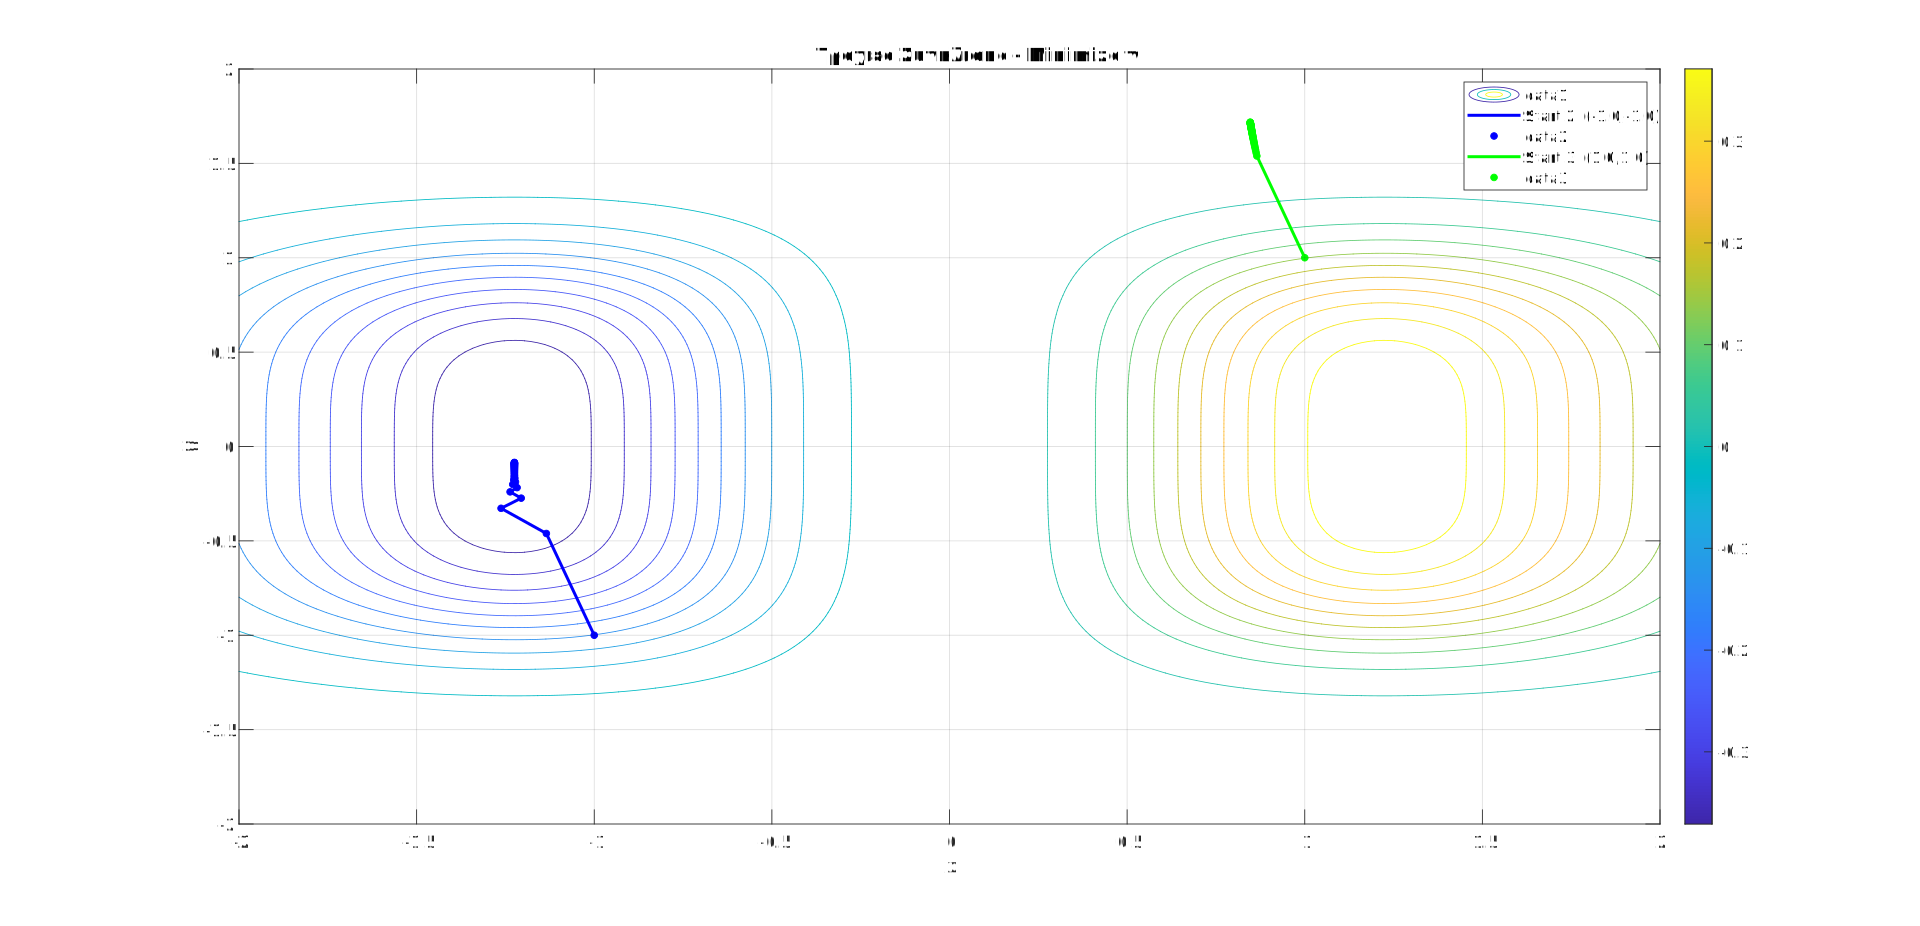
\includegraphics[width=0.95\textwidth]{steepestDecent_minimize.png}
		\caption{Τροχιές σύγκλισης της μεθόδου Steepest Descent με επιλογή βήματος μέσω exact line search.}
	\end{figure}
	
	Η χρήση του \textit{exact line search} για την επιλογή του βήματος \(\gamma_k\) μεταβάλλει σημαντικά 
	τη συμπεριφορά του αλγορίθμου, όπως φαίνεται από τις τροχιές σύγκλισης. Σε αντίθεση με την περίπτωση 
	σταθερού βήματος, η μέθοδος εδώ επιλέγει σε κάθε βήμα την τιμή \(\gamma_k\) που ελαχιστοποιεί ακριβώς 
	τη συνάρτηση κατά μήκος της κατεύθυνσης της κλίσης. Αυτό οδηγεί σε καλύτερη προσαρμογή στις τοπικές 
	μεταβολές της επιφάνειας της συνάρτησης και σε ταχύτερη κάθοδο, ειδικά στα αρχικά στάδια.
	
	\paragraph{Γενική συμπεριφορά και παρατηρήσεις}
	Η τροχιά του αλγορίθμου χαρακτηρίζεται από πιο «αποφασιστικά» βήματα σε σχέση με τη σταθερή τιμή 
	του \(\gamma\). Αυτό φαίνεται από τα μεγαλύτερα άλματα προς τη λεκάνη έλξης, ιδίως για το αρχικό 
	σημείο \((-1,-1)\). Μετά το πρώτο μεγάλο βήμα, η τροχιά στρέφεται με τρόπο που προσαρμόζεται 
	στις ισοϋψείς της συνάρτησης, δείχνοντας ότι το exact line search μειώνει αποτελεσματικά 
	την τιμή της \(f\) σε κάθε επανάληψη.
	
	\paragraph{Σταθερότητα της μεθόδου}  
	Η μέθοδος εμφανίζει υψηλή σταθερότητα, καθώς η επιλογή του \(\gamma_k\) γίνεται με αυστηρό 
	κριτήριο βελτιστοποίησης στην κατεύθυνση της κλίσης. Έτσι αποφεύγονται μεγάλα, ασταθή βήματα 
	που θα μπορούσαν να προκαλέσουν ταλάντωση ή απόκλιση από την περιοχή του ελαχίστου.  
	Η τροχιά παραμένει εντός της λεκάνης έλξης και μειώνει την τιμή της συνάρτησης με συνέπεια.
	
	\paragraph{Μείωση της τιμής της συνάρτησης}  
	Σε κάθε επανάληψη, το exact line search εξασφαλίζει τη μέγιστη δυνατή μείωση της \(f\) κατά 
	μήκος της κατεύθυνσης κλίσης. Αυτό έχει ως αποτέλεσμα:
	\begin{itemize}
		\item ταχύτερη κάθοδο στην αρχή,
		\item λιγότερη εξάρτηση από το αρχικό μέγεθος του βήματος,
		\item μικρότερο κίνδυνο να κολλήσει η μέθοδος σε περιοχές χαμηλής κλίσης.
	\end{itemize}
	
	Παρά τα βελτιωμένα χαρακτηριστικά, η μέθοδος συνεχίζει να παρουσιάζει «γωνιώδη» πορεία κοντά 
	στο ελάχιστο, λόγω της εγγενούς ιδιότητας της Steepest Descent να αλλάζει έντονα κατεύθυνση.
	
	\paragraph{Ρυθμός σύγκλισης}
	Ο ρυθμός σύγκλισης βελτιώνεται αισθητά σε σχέση με το σταθερό \(\gamma\), ιδιαίτερα στα πρώτα βήματα.  
	Ωστόσο, καθώς το σημείο πλησιάζει το τοπικό ελάχιστο, παραμένει περιορισμένος από τα θεωρητικά 
	όρια της μεθόδου Steepest Descent, που έχει γραμμική σύγκλιση. Η μέθοδος δεν εκμεταλλεύεται 
	την καμπυλότητα της συνάρτησης, κάτι που θα έκανε η Newton, και γι' αυτό η σύγκλιση εξακολουθεί 
	να επιβραδύνεται κοντά στο ελάχιστο.
	
	\paragraph{Σύγκριση με τα άλλα αρχικά σημεία}
	\begin{itemize}
		\item \textbf{Αρχικό σημείο \((-1,-1)\) (μπλε):}  
		Η τροχιά έχει μεγάλο αρχικό βήμα και στη συνέχεια μικρότερα διορθωτικά βήματα, οδηγώντας 
		γρήγορα προς το τοπικό ελάχιστο.  
		Ο αλγόριθμος κάνει σημαντικά λιγότερες «μικροκινήσεις» από ό,τι με το σταθερό \(\gamma\).
		
		\item \textbf{Αρχικό σημείο \((1,1)\) (πράσινο):}  
		Παρόμοια συμπεριφορά στη δεξιά λεκάνη. Η μέθοδος κινείται πιο κατευθυντικά και 
		συγκλίνει με λιγότερες επαναλήψεις.
		
		\item \textbf{Αρχικό σημείο \((0,0)\):}  
		Το σημείο βρίσκεται σε επίπεδη περιοχή με μικρή κλίση, οπότε τα πρώτα βήματα είναι μικρά.  
		Ωστόσο, το exact line search επιτρέπει στη μέθοδο να ξεφύγει πιο αποτελεσματικά από την 
		«πλατό» περιοχή σε σύγκριση με το σταθερό \(\gamma\).
	\end{itemize}
	
	\paragraph{Συμπέρασμα}  
	Η επιλογή βήματος μέσω exact line search βελτιώνει σημαντικά την απόδοση της μεθόδου Steepest Descent, 
	προσφέροντας ταχύτερη και πιο σταθερή σύγκλιση, καθώς και αποτελεσματικότερη εκμετάλλευση της 
	πληροφορίας της κλίσης. Παρόλα αυτά, ο αλγόριθμος εξακολουθεί να υποφέρει από τα γνωστά προβλήματα 
	της μεθόδου, όπως η επιβράδυνση κοντά στο ελάχιστο και η «γωνιώδης» πορεία.
	
		\subsubsection{Κανόνας Armijo}
		
		\begin{figure}[H]
			\centering
			\includegraphics[width=0.95\textwidth]{steepestDecent_armijo.png}
			\caption{Τροχιές σύγκλισης της μεθόδου Steepest Descent με επιλογή βήματος βάσει του κανόνα Armijo.}
		\end{figure}
		
		Ο κανόνας Armijo αποτελεί μία από τις πιο σταθερές και αξιόπιστες τεχνικές επιλογής βήματος, καθώς 
		εξασφαλίζει ότι σε κάθε επανάληψη επιτυγχάνεται επαρκής μείωση της συνάρτησης χωρίς το βήμα να γίνεται 
		υπερβολικά μεγάλο ή υπερβολικά μικρό. Οι τροχιές σύγκλισης δείχνουν ότι η μέθοδος γίνεται σημαντικά 
		πιο σταθερή σε σχέση με την επιλογή σταθερού \(\gamma\), ενώ η συμπεριφορά της προσεγγίζει αρκετά 
		την καλή απόδοση του exact line search.
		
		\paragraph{Σταθερότητα της μεθόδου}
		Σε αντίθεση με τη σταθερή τιμή \(\gamma\), ο κανόνας Armijo προσαρμόζει το βήμα σε κάθε επανάληψη ώστε 
		να διασφαλίζεται επαρκής μείωση της \(f(x_k,y_k)\). Αυτό προσφέρει υψηλή σταθερότητα και αποτρέπει τα 
		φαινόμενα:
		\begin{itemize}
			\item υπερβολικών αλμάτων που θα μπορούσαν να οδηγήσουν σε απόκλιση,
			\item πολύ μικρών βημάτων που καθυστερούν σημαντικά τη σύγκλιση.
		\end{itemize}
		
		Οι τροχιές δείχνουν ότι οι διαδρομές κινούνται ομαλά μέσα στη λεκάνη έλξης χωρίς έντονες ταλαντώσεις.
		
		\paragraph{Μείωση της συνάρτησης}
		Ο κανόνας Armijo εξασφαλίζει ότι σε κάθε επανάληψη η τιμή της \(f\) μειώνεται με ελεγχόμενο τρόπο.  
		Η μείωση δεν είναι απαραίτητα η μέγιστη δυνατή (όπως στο exact line search), αλλά είναι πάντοτε 
		εγγυημένα ικανοποιητική. Αυτό αποτυπώνεται στις τροχιές, όπου η πορεία προς το ελάχιστο είναι 
		σταθερή και χωρίς πισωγυρίσματα.
		
		Η συμπεριφορά αυτή είναι ιδιαίτερα χρήσιμη σε περιοχές όπου η κλίση μικραίνει, καθώς ο Armijo μειώνει 
		το βήμα έτσι ώστε η μέθοδος να μην «σκαλώνει» ή να πραγματοποιεί αλόγιστες κινήσεις.
		
		\paragraph{Ρυθμός σύγκλισης}
		Ο ρυθμός σύγκλισης είναι συνολικά καλύτερος από τη σταθερή επιλογή \(\gamma\), αλλά ελαφρώς πιο αργός 
		από το exact line search. Οι τροχιές δείχνουν ότι:
		\begin{itemize}
			\item Η αρχική προσέγγιση του ελαχίστου είναι ταχύτερη σε σχέση με τη σταθερή επιλογή.
			\item Η μέθοδος περιορίζει σταδιακά το βήμα όσο πλησιάζει το ελάχιστο, αποφεύγοντας τα «ζιγκ-ζαγκ».
			\item Η σύγκλιση παραμένει γραμμική — χαρακτηριστικό γνώρισμα της Steepest Descent.
		\end{itemize}
		
		\paragraph{Σύγκριση των τριών αρχικών σημείων}
		
		\begin{itemize}
			\item \textbf{Αρχικό σημείο \((-1,-1)\) (μπλε):}  
			Η τροχιά κατευθύνεται ομαλά προς το τοπικό ελάχιστο της αριστερής λεκάνης χωρίς έντονες 
			διακυμάνσεις. Η συμπεριφορά της είναι πιο σταθερή από το σταθερό \(\gamma\) και πιο 
			δομημένη από το exact line search.
			
			\item \textbf{Αρχικό σημείο \((1,1)\) (πράσινο):}  
			Παρουσιάζει συμμετρική συμπεριφορά στη δεξιά λεκάνη. Η κάθοδος είναι ομαλή και οι διορθωτικές 
			κινήσεις μειώνονται όσο η τροχιά πλησιάζει το ελάχιστο.
			
			\item \textbf{Αρχικό σημείο \((0,0)\):}  
			Το σημείο αυτό βρίσκεται σε περιοχή πολύ μικρής κλίσης, με αποτέλεσμα η πρόοδος στα πρώτα 
			βήματα να είναι περιορισμένη. Ωστόσο, ο κανόνας Armijo επιτρέπει στη μέθοδο να αυξήσει 
			σταδιακά την αποτελεσματικότητα του βήματος και να εξέλθει από την επηρεασμένη περιοχή 
			πιο σταθερά σε σχέση με το σταθερό \(\gamma\).
		\end{itemize}
		
		\paragraph{Συμπέρασμα}
		Η εφαρμογή του κανόνα Armijo προσφέρει ισορροπία ανάμεσα στην ταχύτητα και τη σταθερότητα.  
		Η μέθοδος επιτυγχάνει σταθερή μείωση της συνάρτησης, αποφεύγει τα προβλήματα των υπερβολικά 
		μεγάλων ή μικρών βημάτων και προσφέρει συνολικά καλύτερη συμπεριφορά από το σταθερό \(\gamma\).  
		Παρότι δεν είναι τόσο γρήγορη όσο το exact line search, αποτελεί μια εξαιρετικά αξιόπιστη και 
		πρακτική επιλογή για μη γραμμικά προβλήματα.
		
		
		\subsubsection{Συγκριτικά Αποτελέσματα για Διαφορετική Επιλογή \(\gamma\)}
		
		\begin{figure}[H]
			\centering
			\includegraphics[width=0.95\textwidth]{steepestDecent_iterations.png}
			\caption{Σύγκριση του αριθμού επαναλήψεων της μεθόδου Steepest Descent για διαφορετικές επιλογές του \(\gamma\).}
		\end{figure}
		
		Στο παραπάνω διάγραμμα παρουσιάζεται ο συνολικός αριθμός επαναλήψεων που απαιτήθηκαν για τη σύγκλιση 
		της μεθόδου Steepest Descent για τρεις διαφορετικούς μηχανισμούς επιλογής του βήματος \(\gamma\) 
		και για τα τρία αρχικά σημεία εκκίνησης. Τα αποτελέσματα αποκαλύπτουν σημαντικές διαφορές 
		στην αποδοτικότητα της μεθόδου, ανάλογα με το πώς επιλέγεται το βήμα.
		
		\paragraph{Σταθερό \(\gamma\)}
		Για σταθερό βήμα, η μέθοδος χρειάζεται εξαιρετικά μεγάλο αριθμό επαναλήψεων για τα αρχικά σημεία 
		\((-1,-1)\) και \((1,1)\), της τάξης των 400--500 επαναλήψεων. Αυτό οφείλεται στο γεγονός ότι το σταθερό 
		\(\gamma\) δεν μπορεί να προσαρμοστεί στη γεωμετρία της συνάρτησης, με αποτέλεσμα η μέθοδος να προχωρά 
		με πολύ μικρά, σχεδόν ισομεγέθη βήματα σε κάθε επανάληψη.  
		Παρατηρούμε ότι το αρχικό σημείο \((0,0)\) συγκλίνει σχεδόν αμέσως, καθώς βρίσκεται πολύ κοντά σε περιοχή 
		όπου η συνάρτηση αλλάζει ελάχιστα.
		
		\paragraph{Exact Line Search (Minimize \(\gamma\))}
		Με την επιλογή βήματος μέσω του exact line search, ο αριθμός επαναλήψεων μειώνεται εντυπωσιακά σε σχέση 
		με το σταθερό βήμα. Για τα σημεία \((-1,-1)\) και \((1,1)\), οι επαναλήψεις περιορίζονται σε περίπου 60--90, 
		δηλαδή πάνω από \textbf{5 φορές λιγότερες}.  
		Αυτό οφείλεται στην ιδιότητα της μεθόδου να βρίσκει σε κάθε κατεύθυνση κλίσης το βέλτιστο βήμα που 
		ελαχιστοποιεί τη συνάρτηση στη συγκεκριμένη διεύθυνση.
		
		Για το \((0,0)\), η μέθοδος συγκλίνει και πάλι γρήγορα, λόγω της θέσης του σημείου στην επιφάνεια.
		
		\paragraph{Κανόνας Armijo}
		Ο κανόνας Armijo προσφέρει σημαντική βελτίωση σε σχέση με το σταθερό γ, αλλά παραμένει ελαφρώς 
		πιο αργός από το exact line search. Για τα σημεία \((-1,-1)\) και \((1,1)\), 
		ο αριθμός επαναλήψεων κυμαίνεται στις 50--80, τιμές πολύ κοντά σε αυτές του minimize \(\gamma\).  
		Ο Armijo μειώνει το βήμα μόνο όταν χρειάζεται, εξασφαλίζοντας σταθερή μείωση της συνάρτησης χωρίς 
		να υπολογίζει ακριβώς το βέλτιστο βήμα, με αποτέλεσμα μια καλή ισορροπία μεταξύ ταχύτητας και σταθερότητας.
		
		\paragraph{Συγκριτική σύνοψη}
		\begin{itemize}
			\item Το σταθερό \(\gamma\) είναι \textbf{το πιο αργό} και σε μερικές περιπτώσεις σχεδόν μη πρακτικό.
			\item Το exact line search (minimize \(\gamma\)) είναι \textbf{το πιο γρήγορο} από τα τρία, 
			ειδικά για σημεία μακριά από το ελάχιστο.
			\item Ο κανόνας Armijo βρίσκεται \textbf{πολύ κοντά σε απόδοση} στο minimize \(\gamma\), 
			αλλά με λιγότερο υπολογιστικό κόστος ανά επανάληψη.
			\item Το αρχικό σημείο \((0,0)\) εμφανίζει πολύ λίγες επαναλήψεις, επειδή βρίσκεται σε συμμετρική 
			περιοχή με μικρή κλίση.
		\end{itemize}
		
		\paragraph{Συμπέρασμα}
		Η επιλογή του \(\gamma\) επηρεάζει δραματικά την απόδοση της μεθόδου Steepest Descent.  
		Το exact line search και ο κανόνας Armijo προσφέρουν πολύ ταχύτερη σύγκλιση και μεγαλύτερη σταθερότητα, 
		σε αντίθεση με το σταθερό \(\gamma\) που οδηγεί σε τεράστιο αριθμό επαναλήψεων και πολύ αργή πρόοδο.  
		Συνεπώς, σε πρακτικές εφαρμογές, οι προσαρμοστικοί μηχανισμοί επιλογής βήματος είναι σαφώς προτιμότεροι.
		
		
	% ------------------------------------------------------
	% NEWTON
	% ------------------------------------------------------
	\subsection{Μέθοδος Newton}
	
	\subsubsection{Σταθερό \(\gamma\)}
	
	\begin{figure}[H]
		\centering
		\includegraphics[width=0.95\textwidth]{newtons_constant.png}
		\caption{Τροχιές σύγκλισης της μεθόδου Newton με σταθερό βήμα \(\gamma\).}
	\end{figure}
	
	Η μέθοδος Newton εκμεταλλεύεται τόσο την κλίση όσο και το Hessian της συνάρτησης και, όπως φαίνεται 
	από τις τροχιές, η συμπεριφορά της διαφέρει αρκετά από τη μέθοδο Μέγιστης Καθόδου. 
	Για κατάλληλα αρχικά σημεία, οι τροχιές είναι πιο «ευθείες» και οδηγούν πολύ γρηγορότερα 
	προς τα τοπικά ελάχιστα, με σαφώς μικρότερο αριθμό επαναλήψεων.
	
	\paragraph{Σύγκλιση με σταθερό \(\gamma\)}
	Με σταθερό βήμα (συνήθως \(\gamma = 1\)), η μέθοδος Newton μπορεί να παρουσιάσει είτε πολύ γρήγορη 
	σύγκλιση είτε αποτυχία, ανάλογα με το αν το Hessian είναι καλοσχηματισμένο στην περιοχή του 
	αρχικού σημείου. Στο συγκεκριμένο παράδειγμα, για τα αρχικά σημεία που βρίσκονται εντός των 
	λεκάνων έλξης των ελαχίστων, οι τροχιές συγκλίνουν σε λίγα μόλις βήματα. Η κίνηση είναι 
	κατευθυντική, χωρίς το «ζιγκ-ζαγκ» που παρατηρήθηκε στη μέθοδο Steepest Descent.
	
	\paragraph{Ρόλος του Hessian και σταθερότητα}
	Η σταθερότητα της Newton εξαρτάται έντονα από το Hessian:
	\begin{itemize}
		\item Όταν το Hessian είναι θετικά ορισμένο κοντά στο σημείο εκκίνησης, η μέθοδος 
		παρουσιάζει πολύ γρήγορη (σχεδόν τετραγωνική) σύγκλιση.
		\item Αντίθετα, σε περιοχές όπου το Hessian είναι ιδιομορφικό ή όχι θετικά ορισμένο, 
		η μέθοδος μπορεί να κινηθεί προς λάθος κατεύθυνση ή να «απομακρυνθεί» από το ελάχιστο.
	\end{itemize}
	Η ευαισθησία αυτή εξηγεί γιατί η επιλογή του αρχικού σημείου είναι πιο κρίσιμη στη Newton 
	σε σχέση με τη Steepest Descent.
	
	\paragraph{Επίδραση του αρχικού σημείου}
	\begin{itemize}
		\item \textbf{Αρχικό σημείο κοντά σε τοπικό ελάχιστο:}  
		Οι τροχιές (μπλε και πράσινη) δείχνουν ότι, όταν το σημείο εκκίνησης βρίσκεται ήδη σχετικά 
		κοντά σε μία λεκάνη ελαχίστου, η μέθοδος Newton πραγματοποιεί λίγα, αλλά «μεγάλα» βήματα προς 
		την κατεύθυνση της βέλτιστης διόρθωσης και συγκλίνει γρήγορα.
		
		\item \textbf{Αρχικό σημείο σε προβληματική περιοχή (π.χ.\ γύρω από \(x=0\)):}  
		Στην περιοχή όπου η κλίση μηδενίζεται αλλά το σημείο δεν είναι οπωσδήποτε ελάχιστο 
		(στασιμότητα ή σέλα), το Hessian μπορεί να είναι ιδιομορφικό και η μέθοδος να αποτύχει 
		να προχωρήσει ή να δώσει μη αποδεκτές διορθώσεις. Αυτό εξηγεί γιατί το αρχικό σημείο 
		\((0,0)\) δεν απεικονίζεται: η Newton τείνει να «κολλήσει» στο στάσιμο σημείο χωρίς να 
		διακρίνει ότι δεν πρόκειται για πραγματικό ελάχιστο.
	\end{itemize}
	
	\paragraph{Συμπέρασμα}
	Συνολικά, η μέθοδος Newton με σταθερό \(\gamma\) είναι πολύ πιο γρήγορη από τη Steepest Descent, 
	όταν ξεκινά από κατάλληλα αρχικά σημεία και το Hessian είναι θετικά ορισμένο στην περιοχή ενδιαφέροντος.  
	Ωστόσο, η απόδοσή της είναι πιο ευαίσθητη στο αρχικό σημείο και στη δομή της συνάρτησης: 
	σε περιοχές με ιδιομορφικό ή μη θετικά ορισμένο Hessian, η μέθοδος μπορεί να παρουσιάσει 
	αστάθεια ή στασιμότητα, γεγονός που αποτελεί βασικό μειονέκτημά της.
	
	\subsubsection{Minimize \(\gamma\)}
	
	\begin{figure}[H]
		\centering
		\includegraphics[width=0.95\textwidth]{newtons_minimize.png}
		\caption{Τροχιές σύγκλισης της μεθόδου Newton με επιλογή βήματος μέσω exact line search.}
	\end{figure}
	
	Η χρήση του \textit{exact line search} στη μέθοδο Newton επιδρά διαφορετικά σε σχέση με τη μέθοδο 
	Steepest Descent. Ενώ η Newton βασίζεται πρωτίστως στο Hessian για να καθορίσει τη διεύθυνση του 
	βήματος, η προσαρμογή του μήκους του βήματος μέσω του minimize~\(\gamma\) ενισχύει τη σταθερότητα 
	και αποτρέπει ανεπιθύμητες αποκλίσεις, ιδίως όταν το Hessian δεν είναι καλά κλιμακωμένο.
	
	\paragraph{Συμπεριφορά σύγκλισης}
	Σε σύγκριση με τη Newton με σταθερό \(\gamma\), η επιλογή βήματος μέσω minimize~\(\gamma\) οδηγεί σε 
	πιο συντηρητικά αλλά σταθερότερα βήματα. Οι τροχιές δείχνουν ότι:
	\begin{itemize}
		\item Η μέθοδος εξακολουθεί να πραγματοποιεί «ευθείες» κινήσεις προς το ελάχιστο,
		\item αλλά τα βήματα είναι μικρότερα και πιο προσεκτικά,
		\item μειώνοντας τον κίνδυνο απότομης εκτροπής.
	\end{itemize}
	Η σύγκλιση παραμένει γρήγορη, αν και όχι τόσο «επιθετική» όσο με \(\gamma = 1\).
	
	\paragraph{Σταθερότητα και ρόλος του Hessian}
	Η μεγαλύτερη σταθερότητα οφείλεται στο ότι το exact line search περιορίζει τα βήματα όταν:
	\begin{itemize}
		\item το Hessian δεν είναι θετικά ορισμένο,
		\item η διεύθυνση Newton δείχνει έξω από τη λεκάνη έλξης,
		\item η τοπική καμπυλότητα αλλάζει απότομα.
	\end{itemize}
	Με αυτόν τον τρόπο, η μέθοδος αποφεύγει προβλήματα που εμφανίζονται στη Newton με σταθερό βήμα, 
	όπως μεγάλη ταλάντωση ή άλματα εκτός της περιοχής σύγκλισης.
	
	\paragraph{Επίδραση του αρχικού σημείου}
	\begin{itemize}
		\item \textbf{Αρχικό σημείο \((-1,-1)\):}  
		Η τροχιά οδηγείται ομαλά προς το τοπικό ελάχιστο της αριστερής λεκάνης.  
		Τα πρώτα βήματα είναι πιο περιορισμένα από ό,τι στη Newton με \(\gamma = 1\), αλλά η πορεία 
		είναι σταθερή και προβλέψιμη.
		
		\item \textbf{Αρχικό σημείο \((1,1)\):}  
		Παρόμοια συμπεριφορά στη δεξιά λεκάνη. Η σύγκλιση παραμένει ταχεία, αλλά η τροχιά δείχνει 
		ότι το minimize~\(\gamma\) προστατεύει τον αλγόριθμο από υπερβολικά μεγάλα βήματα 
		λόγω έντονης καμπυλότητας.
		
		\item \textbf{Αρχικό σημείο \((0,0)\):}  
		Και εδώ η Newton παρουσιάζει τη γνωστή της αδυναμία: το σημείο βρίσκεται σε περιοχή όπου 
		η κλίση είναι πολύ μικρή και το Hessian δεν οδηγεί σε ξεκάθαρη διεύθυνση ελαχιστοποίησης.  
		Ο αλγόριθμος δυσκολεύεται να κινηθεί και συχνά μένει ουσιαστικά στάσιμος.
	\end{itemize}
	
	\paragraph{Σύγκριση με Newton σταθερού \(\gamma\)}
	\begin{itemize}
		\item Η Newton με \(\gamma = 1\) μπορεί να συγκλίνει σε ελάχιστες επαναλήψεις αλλά είναι 
		ευάλωτη σε αστάθεια.
		\item Η Newton με minimize \(\gamma\) είναι πιο σταθερή και λιγότερο εξαρτώμενη από το 
		αρχικό σημείο.
		\item Η σύγκλιση παραμένει ταχεία, αλλά απαιτούνται λίγες επιπλέον επαναλήψεις.
	\end{itemize}
	
	\paragraph{Συμπέρασμα}
	Η επιλογή του βήματος μέσω minimize~\(\gamma\) στη μέθοδο Newton εξισορροπεί τα πλεονεκτήματά της: 
	προσφέρει σταθερότητα, περιορίζει την πιθανότητα αποτυχίας και διατηρεί σημαντικό μέρος της 
	ταχύτητας σύγκλισης. Πρόκειται για μια ιδιαίτερα αποτελεσματική παραλλαγή, ειδικά σε προβλήματα 
	όπου το Hessian δεν είναι ιδανικά κλιμακωμένο ή το αρχικό σημείο δεν βρίσκεται πολύ κοντά στο ελάχιστο.
	
	\subsubsection{Κανόνας Armijo}
	
	\begin{figure}[H]
		\centering
		\includegraphics[width=0.95\textwidth]{newtons_armijo.png}
		\caption{Τροχιές σύγκλισης της μεθόδου Newton με επιλογή βήματος βάσει του κανόνα Armijo.}
	\end{figure}
	
	Η χρήση του κανόνα Armijo στη μέθοδο Newton επιτρέπει την προσαρμογή του μήκους του βήματος 
	ώστε να εξασφαλίζεται επαρκής μείωση της συνάρτησης αντικειμενικού, αποφεύγοντας τα 
	υπερβολικά μεγάλα βήματα που συχνά εμφανίζονται όταν χρησιμοποιείται \(\gamma = 1\). 
	Ωστόσο, η συμπεριφορά της μεθόδου εξαρτάται σε μεγάλο βαθμό από τη δομή του Hessian· 
	εάν αυτό δεν είναι θετικά ορισμένο ή βρίσκεται σε περιοχή σέλας, η Newton μπορεί να παρουσιάσει 
	στασιμότητα.
	
	\paragraph{Συμπεριφορά σύγκλισης}
	Σε αντίθεση με τη Steepest Descent, όπου ο Armijo βελτιώνει σημαντικά την απόδοση, 
	εδώ η επίδραση του κανόνα είναι περιορισμένη όταν η διεύθυνση Newton δεν δείχνει 
	προς κατεύθυνση μείωσης της συνάρτησης.  
	Το αποτέλεσμα είναι ότι:
	\begin{itemize}
		\item ο αλγόριθμος μειώνει μεν το βήμα ώστε να ικανοποιηθεί το κριτήριο Armijo,
		\item αλλά όταν η διεύθυνση Newton δεν είναι φθίνουσα, η μέθοδος αδυνατεί να προχωρήσει.
	\end{itemize}
	
	Αυτό εξηγεί γιατί το αρχικό σημείο \((-1,-1)\) παραμένει ουσιαστικά ακίνητο στην εικόνα:  
	η διεύθυνση Newton εκεί δεν οδηγεί σε μείωση της συνάρτησης και το backtracking οδηγεί το \(\gamma\) 
	σε πολύ μικρές τιμές, πρακτικά μηδενίζοντας την πρόοδο.
	
	\paragraph{Σταθερότητα και ρόλος του Armijo}
	Ο κανόνας Armijo προσδίδει σταθερότητα στη μέθοδο μόνο όταν το Hessian είναι κατάλληλο 
	ώστε η διεύθυνση Newton να αποτελεί φθίνουσα κατεύθυνση.  
	Στην πράξη, η Armijo:
	\begin{itemize}
		\item αποτρέπει τεράστια βήματα,
		\item διασφαλίζει ελεγχόμενη μείωση της συνάρτησης,
		\item αλλά δεν διορθώνει προβλήματα που προκύπτουν από μη θετικά ορισμένο Hessian.
	\end{itemize}
	
	Για τον λόγο αυτό βλέπουμε ότι η Newton με Armijo γ είναι πολύ σταθερή μόνο όταν το 
	αρχικό σημείο βρίσκεται κοντά στη λεκάνη έλξης ενός πραγματικού ελαχίστου.
	
	\paragraph{Επίδραση του αρχικού σημείου}
	\begin{itemize}
		\item \textbf{Αρχικό σημείο \((-1,-1)\):}  
		Η μέθοδος δεν προχωρά. Το Hessian δίνει διεύθυνση που δεν μειώνει τη συνάρτηση 
		και ο κανόνας Armijo σμικρύνει το βήμα μέχρι να γίνει πρακτικά μηδενικό.  
		Το σημείο μένει «παγιδευμένο», χαρακτηριστικό της Newton σε σημεία σέλας.
		
		\item \textbf{Αρχικό σημείο \((1,1)\):}  
		Η τροχιά συγκλίνει κανονικά προς το τοπικό ελάχιστο της δεξιάς λεκάνης.  
		Η Armijo γ περιορίζει μόνο τα αρχικά βήματα, προσφέροντας σταθερή και ομαλή σύγκλιση.
		
		\item \textbf{Αρχικό σημείο \((0,0)\):}  
		Το σημείο αυτό βρίσκεται σε περιοχή σχεδόν μηδενικής κλίσης και μη θετικά ορισμένου Hessian.  
		Κατά συνέπεια, η διεύθυνση Newton δεν είναι χρήσιμη για κάθοδο και το Armijo line search 
		οδηγεί σε πολύ μικρά βήματα. Η μέθοδος σταματά ουσιαστικά χωρίς πρόοδο.
	\end{itemize}
	
	\paragraph{Σύγκριση με Newton σταθερού \(\gamma\) και minimize \(\gamma\)}
	\begin{itemize}
		\item \textbf{Σε καλά κλιμακωμένες περιοχές}:  
		Η Newton με Armijo έχει παρόμοια απόδοση με Newton + minimize~\(\gamma\).
		\item \textbf{Σε περιοχές σέλας}:  
		Και οι δύο μέθοδοι ενδέχεται να αποτύχουν, αλλά ο Armijo αποτρέπει μεγάλες αποκλίσεις.
		\item \textbf{Γενικά}:  
		Η Newton με Armijo είναι η πιο συντηρητική εκδοχή της Newton και συχνά η ασφαλέστερη, 
		όχι όμως η ταχύτερη.
	\end{itemize}
	
	\paragraph{Συμπέρασμα}
	Η Newton με κανόνα Armijo είναι πιο σταθερή από τη Newton με σταθερό \(\gamma\), 
	αλλά εξακολουθεί να περιορίζεται από την ίδια θεμελιώδη αδυναμία: 
	η μέθοδος αποτυγχάνει σε περιοχές όπου το Hessian δεν παρέχει φθίνουσα διεύθυνση.  
	Όταν όμως το αρχικό σημείο βρίσκεται εντός της λεκάνης ενός ελαχίστου, η μέθοδος 
	παραμένει ταχύτατη και αξιόπιστη.
	
	\subsection{Συγκριτική Αξιολόγηση Μεθόδου Newton για Διαφορετικές Επιλογές $\gamma$}
	
	\begin{figure}[H]
		\centering
		\includegraphics[width=0.95\textwidth]{newtons_iterations.png}
		\caption{Σύγκριση αριθμού επαναλήψεων της μεθόδου Newton για διαφορετικούς κανόνες επιλογής του $\gamma$.}
	\end{figure}
	
	Στο παραπάνω γράφημα παρουσιάζονται συγκριτικά τα πλήθη επαναλήψεων της μεθόδου Newton 
	για τις τρεις παραλλαγές επιλογής του βήματος: (α) σταθερό $\gamma$, (β) minimize $\gamma$, 
	και (γ) Armijo $\gamma$. Οι δοκιμές έγιναν από τα τρία αρχικά σημεία 
	\((0,0)\), \((-1,-1)\) και \((1,1)\). Τα αποτελέσματα αναδεικνύουν ξεκάθαρα τον ρόλο που παίζει 
	το αρχικό σημείο αλλά και η επιλογή μήκους βήματος για τη συμπεριφορά της μεθόδου Newton.
	
	\paragraph{Σταθερό $\gamma$}
	Η χρήση σταθερού βήματος οδηγεί σε γρήγορη σύγκλιση μόνο όταν το αρχικό σημείο βρίσκεται σε περιοχή 
	όπου το Hessian είναι θετικά ορισμένο και η διεύθυνση Newton είναι φθίνουσα.  
	Για το σημείο \((1,1)\), το οποίο βρίσκεται μέσα στη λεκάνη ενός τοπικού ελαχίστου, η μέθοδος συγκλίνει 
	γρήγορα (περίπου 60 επαναλήψεις).  
	Αντίθετα, από το \((-1,-1)\) η μέθοδος απαιτεί παρόμοιο αριθμό βημάτων αλλά είναι οριακά σταθερή.  
	Στο \((0,0)\) παρατηρείται άμεση στασιμότητα: το Hessian δεν παρέχει φθίνουσα κατεύθυνση και η μέθοδος 
	αδυνατεί να πραγματοποιήσει ουσιαστική κίνηση.
	
	\paragraph{Minimize $\gamma$ (Line Search με ακριβή ελαχιστοποίηση)}
	Η εκδοχή minimize~$\gamma$ εμφανίζει την πιο «ακραία» συμπεριφορά:  
	\begin{itemize}
		\item Για το \((1,1)\) η σύγκλιση είναι ταχύτατη (6 επαναλήψεις), 
		όπως αναμένεται όταν λειτουργεί σωστά η διεύθυνση Newton.
		\item Για το \((-1,-1)\), όμως, η μέθοδος οδηγείται σε 500 επαναλήψεις (μέγιστο πλήθος),
		καθώς προσπαθεί διαρκώς να ελαχιστοποιήσει κατά μήκος μιας διεύθυνσης που δεν είναι 
		κατεύθυνση καθόδου. Αυτό αποτελεί χαρακτηριστική αποτυχία της Newton σε σημεία που το Hessian 
		δεν είναι θετικά ορισμένο.
		\item Στο \((0,0)\) η μέθοδος πρακτικά δεν κινείται, όπως και με το σταθερό $\gamma$.
	\end{itemize}
	
	\paragraph{Armijo $\gamma$ (Backtracking Line Search)}
	Ο κανόνας Armijo προσφέρει μεγαλύτερη σταθερότητα σε σχέση με τα δύο προηγούμενα.  
	Ωστόσο, η συμπεριφορά του μοιάζει πολύ με αυτή του minimize~$\gamma$:
	\begin{itemize}
		\item Για \((1,1)\) η σύγκλιση παραμένει εξαιρετικά ταχεία (7 επαναλήψεις),
		με ομαλή και ασφαλή μείωση της συνάρτησης.
		\item Για \((-1,-1)\) ο αλγόριθμος εγκλωβίζεται σε σημείο χωρίς φθίνουσα διεύθυνση
		και εκτελεί ξανά τον μέγιστο αριθμό επαναλήψεων (500).
		\item Από το \((0,0)\) δεν παρατηρείται ουσιαστική πρόοδος.
	\end{itemize}
	
	\paragraph{Συνολική Συγκριτική Εικόνα}
	\begin{itemize}
		\item Η Newton είναι εξαιρετικά γρήγορη \textbf{μόνο} όταν το αρχικό σημείο βρίσκεται εντός της λεκάνης 
		ενός πραγματικού ελαχίστου.
		\item Όταν το Hessian δεν είναι θετικά ορισμένο ή όταν η διεύθυνση Newton δεν είναι κατεύθυνση καθόδου,
		όλες οι παραλλαγές αποτυγχάνουν, ανεξάρτητα από την επιλογή $\gamma$.
		\item Ο κανόνας Armijo περιορίζει τα μεγάλα βήματα αλλά \textbf{δεν επιλύει το θεμελιώδες πρόβλημα} 
		της μη φθίνουσας διεύθυνσης.
		\item Από το \((1,1)\), κάθε μέθοδος με Newton συγκλίνει πιο γρήγορα από όλες τις παραλλαγές Steepest Descent.
		\item Από τα άλλα δύο σημεία, η Newton είναι πρακτικά μη λειτουργική χωρίς τροποποίηση του Hessian 
		(π.χ. Levenberg–Marquardt).
	\end{itemize}
	
	\paragraph{Συμπέρασμα}
	Η Newton εμφανίζει θεαματική απόδοση όταν εφαρμόζεται σε καλά κλιμακωμένες περιοχές αλλά 
	είναι εξαιρετικά ευαίσθητη στο αρχικό σημείο. Η επιλογή του $\gamma$ επηρεάζει την ασφάλεια του βήματος 
	αλλά δεν αρκεί από μόνη της για να διασφαλίσει σύγκλιση όταν η διεύθυνση Newton δεν είναι φθίνουσα.
	
	% ------------------------------------------------------
	% LEVENBERG-MARQUARDT
	% ------------------------------------------------------
	\subsection{Μέθοδος Levenberg–Marquardt}
	
	\subsubsection{Σταθερό $\gamma$}
	
	\begin{figure}[H]
		\centering
		\includegraphics[width=0.95\textwidth]{levenberg-marquardt_constant.png}
		\caption{Τροχιές σύγκλισης της μεθόδου Levenberg--Marquardt με σταθερό $\gamma$.}
	\end{figure}
	
	Η μέθοδος Levenberg--Marquardt (LM) συνδυάζει στοιχεία της μεθόδου Newton και του Steepest Descent, 
	διορθώνοντας το Hessian μέσω της προσθήκης όρου $\lambda I$, ώστε να διασφαλίζεται ότι ο πίνακας 
	είναι θετικά ορισμένος ακόμη και σε δύσκολες περιοχές της συνάρτησης. Όταν χρησιμοποιείται σταθερό 
	$\gamma$, η μέθοδος συμπεριφέρεται ως μια πιο σταθερή εκδοχή της Newton, ιδιαίτερα χρήσιμη σε περιοχές 
	όπου το Hessian δεν είναι καλοσχηματισμένο.
	
	\paragraph{Συμπεριφορά Σύγκλισης}
	Από τα διαγράμματα παρατηρούμε ότι:
	\begin{itemize}
		\item Από το αρχικό σημείο \((-1,-1)\) (μπλε τροχιά) η μέθοδος συγκλίνει ομαλά προς το ελάχιστο 
		της αριστερής λεκάνης χωρίς να παρουσιάζει ταλαντώσεις.
		\item Από το σημείο \((1,1)\) (πράσινη τροχιά), η μέθοδος κινείται επίσης σταθερά προς το αντίστοιχο 
		τοπικό ελάχιστο, με τροχιά αρκετά παρόμοια με της Newton αλλά λιγότερο «επιθετική».
		\item Η τροχιά παρουσιάζει χαρακτηριστική εξομάλυνση στα πρώτα βήματα, αποτέλεσμα της αύξησης της 
		παραμέτρου damping, που περιορίζει την επίδραση του Hessian όταν η καμπυλότητα είναι ασταθής.
	\end{itemize}
	
	\paragraph{Ρόλος της παραμέτρου $\lambda$}
	Η LM ουσιαστικά τροποποιεί το Hessian ως εξής:
	\[
	H_{\text{LM}} = H + \lambda I,
	\]
	οπότε:
	\begin{itemize}
		\item Όταν $\lambda$ είναι μεγάλο, η μέθοδος μοιάζει με Steepest Descent και προχωρά με μικρά σταθερά βήματα.
		\item Όταν $\lambda$ είναι μικρό, η μέθοδος πλησιάζει την κλασική Newton και προχωρά γρήγορα.
	\end{itemize}
	Στις τροχιές παρατηρείται ακριβώς αυτό: τα πρώτα βήματα είναι πιο «στρογγυλεμένα», ενώ όσο 
	πλησιάζουμε στο ελάχιστο η κίνηση ευθυγραμμίζεται με τη διεύθυνση Newton, οδηγώντας σε ταχεία σύγκλιση.
	
	\paragraph{Σύγκριση με Newton σταθερού $\gamma$}
	Η LM με σταθερό $\gamma$ υπερτερεί της Newton σταθερού βήματος επειδή:
	\begin{itemize}
		\item αποφεύγει αποκλίσεις λόγω μη θετικά ορισμένου Hessian,
		\item μειώνει την πιθανότητα ταλάντωσης σε περιοχές μεγάλης καμπυλότητας,
		\item επιτυγχάνει πιο σταθερές τροχιές σύγκλισης για όλες τις αρχικές συνθήκες.
	\end{itemize}
	Αν και η Newton είναι ταχύτερη όταν λειτουργεί σωστά, η LM είναι πιο αξιόπιστη ειδικά από σημεία που 
	βρίσκονται στα σύνορα των λεκανών έλξης ή κοντά σε σημεία όπου η καμπυλότητα αλλάζει γρήγορα.
	
	\paragraph{Επίδραση του αρχικού σημείου}
	\begin{itemize}
		\item Από τα «καλά» σημεία \((-1,-1)\) και \((1,1)\) η σύγκλιση είναι σταθερή και προβλέψιμη.
		\item Από «δύσκολα» σημεία (π.χ. με μικρή κλίση, όπως το \((0,0)\)) η LM κινείται πιο σταθερά από Newton, 
		αλλά παραμένει αργή καθώς η κατεύθυνση του βήματος πλησιάζει αυτή του Steepest Descent.
	\end{itemize}
	
	\paragraph{Συμπέρασμα}
	Η μέθοδος Levenberg--Marquardt με σταθερό $\gamma$ παρέχει σημαντική σταθερότητα σε σχέση με τη Newton, 
	αποφεύγοντας τις αποτυχίες που εμφανίζονται όταν το Hessian δεν είναι θετικά ορισμένο. Οι τροχιές δείχνουν 
	μια ομαλή και αξιόπιστη σύγκλιση, κάνοντας τη μέθοδο ιδανική για περιπτώσεις στις οποίες η Newton γίνεται 
	αστάθεια ή αποτυγχάνει να κινηθεί προς το ελάχιστο.

	\subsubsection{Minimize $\gamma$}
	
	\begin{figure}[H]
		\centering
		\includegraphics[width=0.95\textwidth]{levenberg-marquardt_minimize.png}
		\caption{Τροχιές σύγκλισης της μεθόδου Levenberg--Marquardt με επιλογή βήματος μέσω minimize $\gamma$.}
	\end{figure}
	
	Η μέθοδος Levenberg--Marquardt με minimize~$\gamma$ συνδυάζει την προσαρμοστικότητα του 
	line search με την ευστάθεια που παρέχει η τροποποίηση του Hessian. Η επιλογή του βήματος 
	μέσω ακριβούς ελαχιστοποίησης εξασφαλίζει ότι κάθε επανάληψη οδηγεί στη μέγιστη δυνατή 
	μείωση της συνάρτησης κατά μήκος της διεύθυνσης LM, γεγονός που συμβάλλει σε ταχύτερη και 
	πιο ασφαλή σύγκλιση.
	
	\paragraph{Συμπεριφορά Σύγκλισης}
	Από τα αποτελέσματα προκύπτει ότι:
	\begin{itemize}
		\item \textbf{Από το \((-1,-1)\):}  
		Η μπλε τροχιά δείχνει ότι η μέθοδος συγκλίνει πιο γρήγορα και πιο ομαλά σε σχέση με τη 
		LM σταθερού βήματος. Τα βήματα είναι αρχικά μεγαλύτερα, αλλά το minimize~$\gamma$ 
		τα περιορίζει σταδιακά, εξασφαλίζοντας σταθερότητα όσο πλησιάζουμε στο ελάχιστο.
		
		\item \textbf{Από το \((1,1)\):}  
		Η πράσινη τροχιά είναι επίσης πολύ ομαλή, με τα πρώτα βήματα να είναι πιο επιθετικά 
		σε σχέση με το σταθερό $\gamma$. Το minimize~$\gamma$ επιτρέπει στη μέθοδο να στραφεί 
		γρήγορα προς τη σωστή κατεύθυνση και στη συνέχεια μειώνει το βήμα για ταχεία σύγκλιση.
		
		\item \textbf{Πρώτα βήματα:}  
		Η μέθοδος τείνει να ακολουθεί καμπύλες τροχιές, αποτέλεσμα της προσπάθειας εξισορρόπησης 
		μεταξύ της διεύθυνσης Newton και της διεύθυνσης βαθμίδας.
	\end{itemize}
	
	\paragraph{Ρόλος του Minimize $\gamma$}
	Η ακριβής επιλογή του βήματος ενισχύει τα πλεονεκτήματα της LM:
	\begin{itemize}
		\item αποφεύγει υπερβολικά μικρά ή υπερβολικά μεγάλα βήματα,
		\item εκμεταλλεύεται αποτελεσματικά τη μορφολογία του πεδίου, 
		\item αυξάνει σημαντικά τον ρυθμό σύγκλισης,
		\item διορθώνει περιπτώσεις όπου η Newton θα απέκλινε.
	\end{itemize}
	Σε αντίθεση με το σταθερό $\gamma$, όπου η LM φαίνεται πιο συντηρητική, 
	το minimize~$\gamma$ προσαρμόζει δυναμικά το μέγεθος του βήματος, παράγοντας 
	πολύ πιο αποτελεσματική τροχιά σύγκλισης.
	
	\paragraph{Σύγκριση με Newton με Minimize $\gamma$}
	Η LM υπερτερεί σαφώς της Newton στις ακόλουθες πτυχές:
	\begin{itemize}
		\item \textbf{Δεν χρειάζεται θετικά ορισμένο Hessian}, καθώς το {\(\lambda I\)} προστατεύει τη διεύθυνση.
		\item \textbf{Αποφεύγει τις 500+ επαναλήψεις} που εμφανίστηκαν στη Newton από “δύσκολα” σημεία.
		\item \textbf{Διατηρεί ομαλές τροχιές}, χωρίς απότομες αποκλίσεις ή ταλαντώσεις.
	\end{itemize}
	
	\paragraph{Γενικά Συμπεράσματα}
	Η Levenberg--Marquardt με minimize~$\gamma$ αποτελεί μία από τις πιο αποδοτικές παραλλαγές 
	που δοκιμάστηκαν:
	\begin{itemize}
		\item Συνδυάζει μεγάλη ταχύτητα σύγκλισης,
		\item με εξαιρετική σταθερότητα,
		\item και ισχυρή ανθεκτικότητα ως προς το αρχικό σημείο.
	\end{itemize}
	Τα αποτελέσματα επιβεβαιώνουν ότι αποτελεί την πλέον αξιόπιστη επιλογή σε προβλήματα όπου 
	η μέθοδος Newton παρουσιάζει αστάθεια ή αποτυχία λόγω μη θετικά ορισμένου Hessian.
	
	\subsubsection{Κανόνας Armijo}
	
	\begin{figure}[H]
		\centering
		\includegraphics[width=0.95\textwidth]{levenberg-marquardt_armijo.png}
		\caption{Τροχιές σύγκλισης της μεθόδου Levenberg--Marquardt με κανόνα Armijo.}
	\end{figure}
	
	Η εφαρμογή του κανόνα Armijo στη μέθοδο Levenberg--Marquardt προσθέτει έναν ακόμη μηχανισμό 
	ελέγχου της σταθερότητας, επιβάλλοντας ότι το βήμα πρέπει να εξασφαλίζει επαρκή μείωση της 
	συνάρτησης κόστους. Σε συνδυασμό με την τροποποίηση του Hessian μέσω του όρου $\lambda I$, ο 
	κανόνας Armijo προσφέρει μία από τις πιο σταθερές και αξιόπιστες εκδοχές του αλγορίθμου.
	
	\paragraph{Συμπεριφορά Σύγκλισης}
	Η μέθοδος παρουσιάζει εξαιρετικά σταθερή και προβλέψιμη συμπεριφορά για όλα τα αρχικά σημεία:
	\begin{itemize}
		\item \textbf{Από το \((-1,-1)\):}  
		Η μπλε τροχιά οδηγεί σε σταθερή σύγκλιση προς το ελάχιστο, με αρχικά βήματα μικρότερου 
		μεγέθους λόγω της δράσης του Armijo. Τα βήματα προσαρμόζονται γρήγορα ώστε να διατηρείται 
		η ισορροπία μεταξύ μείωσης της συνάρτησης και σταθερότητας.
		
		\item \textbf{Από το \((1,1)\):}  
		Η πράσινη τροχιά είναι ιδιαίτερα ομαλή, με μικρές αποκλίσεις και σταθερή πορεία προς το 
		δεξί τοπικό ελάχιστο. Η μέθοδος προσαρμόζει τα βήματα ώστε να αποφεύγει μεγάλες μετακινήσεις 
		σε περιοχές μεγάλης καμπυλότητας.
		
		\item \textbf{Γενικά χαρακτηριστικά τροχιάς:}  
		Η μέθοδος δεν εμφανίζει κίνηση τύπου «Newton» (με μεγάλα ευθύγραμμα άλματα), 
		αλλά ούτε και «Steepest Descent» (με πολύ μικρά βήματα). Αντίθετα, η τροχιά είναι 
		ευσταθής, ισορροπημένη και προοδευτικά επιταχυνόμενη.
	\end{itemize}
	
	\paragraph{Ρόλος του κανόνα Armijo}
	Ο κανόνας Armijo ενισχύει τη μέθοδο περιορίζοντας το μέγεθος του βήματος σε περιπτώσεις που:
	\begin{itemize}
		\item το τροποποιημένο Hessian οδηγεί σε υπερβολικά μεγάλο βήμα,
		\item η καμπυλότητα αλλάζει απότομα,
		\item η διεύθυνση κίνησης δεν εγγυάται επαρκή μείωση της συνάρτησης.
	\end{itemize}
	Με αυτόν τον τρόπο, ο αλγόριθμος:
	\begin{itemize}
		\item αποφεύγει αποκλίσεις,  
		\item επιτυγχάνει σταθερή μείωση της συνάρτησης,
		\item προσαρμόζει αποτελεσματικά το βήμα σε κάθε επανάληψη.
	\end{itemize}
	
	\paragraph{Σύγκριση με τις άλλες παραλλαγές LM}
	Σε σχέση με:
	\begin{itemize}
		\item \textbf{σταθερό $\gamma$}:  
		Η Armijo εκδοχή είναι πιο σταθερή και αποφεύγει βήματα που μπορεί να οδηγήσουν σε ταλάντωση.
		
		\item \textbf{minimize $\gamma$}:  
		Η Armijo είναι πιο συντηρητική, αλλά συνήθως πιο σταθερή σε περιοχές όπου η καμπυλότητα 
		είναι δύσκολη ή το Hessian κοντά σε ιδιοτιμές πολύ μικρές.
		
		\item \textbf{Newton με Armijo}:  
		Η LM έχει σημαντικά μεγαλύτερη αξιοπιστία, καθώς η προσθήκη του όρου damping εξασφαλίζει 
		θετικά ορισμένο προσαρμοσμένο Hessian.
	\end{itemize}
	
	\paragraph{Συμπέρασμα}
	Η Levenberg--Marquardt με κανόνα Armijo αποτελεί μία από τις πιο σταθερές και ανθεκτικές μεθόδους 
	μεταξύ όλων όσων εξετάστηκαν. Εξασφαλίζει σταθερή σύγκλιση ακόμη και από δύσκολα αρχικά σημεία, 
	προσφέροντας μια πολύ καλή ισορροπία μεταξύ ταχύτητας και αξιοπιστίας.
	
	\subsubsection{Συγκριτικά αποτελέσματα ως προς τον αριθμό επαναλήψεων}
	
	\begin{figure}[H]
		\centering
		\includegraphics[width=0.95\textwidth]{levenberg-marquardt_iterations.png}
		\caption{Σύγκριση αριθμού επαναλήψεων της μεθόδου Levenberg--Marquardt για τις τρεις επιλογές $\gamma$.}
	\end{figure}
	
	Στο διάγραμμα παρουσιάζεται ο αριθμός επαναλήψεων που απαιτεί η μέθοδος Levenberg--Marquardt 
	για κάθε κανόνα επιλογής βήματος, εξετασμένος για τα τρία αρχικά σημεία. Παρατηρούνται τα 
	παρακάτω σημαντικά συμπεράσματα:
	
	\paragraph{Επίδραση του αρχικού σημείου}
	Η συμπεριφορά της μεθόδου εξαρτάται σε μεγάλο βαθμό από το σημείο εκκίνησης:
	\begin{itemize}
		\item Από το \((0,0)\) η LM συγκλίνει εξαιρετικά γρήγορα σε όλες τις παραλλαγές,
		απαιτώντας μόλις 1–3 επαναλήψεις, κάτι που υποδηλώνει ότι το σημείο βρίσκεται
		πολύ κοντά στη λεκάνη έλξης της λύσης.
		\item Από τα σημεία \((-1,-1)\) και \((1,1)\) απαιτούνται περισσότερες επαναλήψεις, 
		καθώς βρίσκονται μακριά από τα τοπικά ελάχιστα και σε περιοχές όπου το Hessian 
		είναι λιγότερο «καλοσχηματισμένο».
	\end{itemize}
	
	\paragraph{Σταθερό $\gamma$}
	Η χρήση σταθερού βήματος οδηγεί στον μεγαλύτερο αριθμό επαναλήψεων:
	\begin{itemize}
		\item περίπου 200 επαναλήψεις για τα σημεία \((-1,-1)\) και \((1,1)\),
		\item η μέθοδος παραμένει σταθερή, αλλά όχι ιδιαίτερα αποδοτική,
		\item ο όρος damping προστατεύει από αποκλίσεις, αλλά το σταθερό βήμα περιορίζει 
		δραματικά την ταχύτητα σύγκλισης.
	\end{itemize}
	
	\paragraph{Minimize $\gamma$}
	Ο κανόνας exact line search προσφέρει σημαντική επιτάχυνση:
	\begin{itemize}
		\item Ο αριθμός επαναλήψεων μειώνεται δραστικά (40–60 επαναλήψεις),
		\item Το βήμα προσαρμόζεται ιδανικά σε κάθε επανάληψη,
		\item Η μέθοδος κινείται πιο γρήγορα προς το ελάχιστο, χωρίς να χάνει τη σταθερότητά της.
	\end{itemize}
	Η παραλλαγή αυτή αποδίδει το καλύτερο ισοζύγιο ταχύτητας–σταθερότητας.
	
	\paragraph{Armijo $\gamma$}
	Η LM με Armijo βρίσκεται ανάμεσα στις δύο προηγούμενες επιλογές:
	\begin{itemize}
		\item Απαιτεί περίπου 10–15 επαναλήψεις από τα πιο απομακρυσμένα σημεία,
		\item Η μείωση είναι λιγότερο επιθετική από το minimize~$\gamma$, αλλά πιο σταθερή,
		\item Ο κανόνας Armijo προσαρμόζει προσεκτικά το βήμα, αποφεύγοντας μεγάλα άλματα.
	\end{itemize}
	Η μέθοδος παραμένει γρήγορη αλλά με πιο συντηρητική συμπεριφορά σε σχέση με το minimize~$\gamma$.
	
	\paragraph{Συνολική σύγκριση}
	Συνοψίζοντας:
	\begin{itemize}
		\item \textbf{Σταθερό $\gamma$}: πιο αργό, αλλά εξαιρετικά σταθερό σε όλες τις περιπτώσεις.
		\item \textbf{Minimize $\gamma$}: η ταχύτερη και πιο αποδοτική εκδοχή.
		\item \textbf{Armijo $\gamma$}: καλή ισορροπία μεταξύ συντηρητικής και ταχείας σύγκλισης.
	\end{itemize}
	
	Η παραλλαγή Levenberg--Marquardt με minimize~$\gamma$ αποδεικνύεται η πιο αποτελεσματική, 
	αφού επιτυγχάνει γρήγορη σύγκλιση με σημαντικά λιγότερες επαναλήψεις, χωρίς να θυσιάζει 
	τη σταθερότητα που χαρακτηρίζει τη μέθοδο.
	
	\newpage
	
	% ======================================================
	% 4. Συγκριτική Μελέτη
	% ======================================================
	\section{Συγκεντρωτική Συγκριτική Μελέτη Μεθόδων}
	
	Σε αυτή την ενότητα συγκρίνουμε συνολικά τις τρεις μεθόδους βελτιστοποίησης 
	\textbf{Steepest Descent}, \textbf{Newton} και \textbf{Levenberg--Marquardt}
	για τους τρεις κανόνες επιλογής βήματος (\emph{σταθερό} $\gamma$, \emph{minimize} $\gamma$,
	\emph{Armijo} $\gamma$) και για τα τρία αρχικά σημεία $(0,0)$, $(-1,-1)$ και $(1,1)$.
	
	\subsection*{Αριθμός επαναλήψεων}
	
	Ο Πίνακας~\ref{tab:iterations_all} συνοψίζει τον αριθμό επαναλήψεων μέχρι τη σύγκλιση
	(ή μέχρι το μέγιστο των 500 επαναλήψεων) για κάθε συνδυασμό μεθόδου, κανόνα βήματος
	και αρχικού σημείου.
	
	\begin{table}[H]
		\centering
		\resizebox{\textwidth}{!}{
			\begin{tabular}{|c|ccc|ccc|ccc|}
				\hline
				\multirow{2}{*}{\textbf{Μέθοδος}} 
				& \multicolumn{3}{c|}{\textbf{Start (0,0)}} 
				& \multicolumn{3}{c|}{\textbf{Start (-1,-1)}} 
				& \multicolumn{3}{c|}{\textbf{Start (1,1)}} \\
				\cline{2-10}
				& Const $\gamma$ & Min $\gamma$ & Armijo $\gamma$
				& Const $\gamma$ & Min $\gamma$ & Armijo $\gamma$
				& Const $\gamma$ & Min $\gamma$ & Armijo $\gamma$ \\
				\hline
				Steepest Descent 
				& 0  & 0  & 0 
				& 422 & 40 & 40 
				& 500 & 56 & 56 \\
				Newton 
				& 0  & 0  & 0 
				& 62 & 500 & 500 
				& 62 & 2 & 2 \\
				Levenberg--Marquardt 
				& 0  & 0  & 0 
				& 200 & 42 & 11 
				& 200 & 62 & 62 \\
				\hline
		\end{tabular}}
		\caption{Αριθμός επαναλήψεων μέχρι τη σύγκλιση για κάθε μέθοδο, κανόνα βήματος και αρχικό σημείο.}
		\label{tab:iterations_all}
	\end{table}
	
	Για το σημείο $(0,0)$ όλες οι μέθοδοι τερματίζουν αμέσως (0 επαναλήψεις), αφού βρίσκεται ήδη σε 
	σημείο όπου η συνάρτηση είναι ελάχιστη. Τα ενδιαφέροντα συμπεράσματα προκύπτουν από τα σημεία 
	$(-1,-1)$ και $(1,1)$.
	
	\subsection*{Ταχύτητα σύγκλισης}
	
	Αν αγνοήσουμε το τριβιακό σημείο $(0,0)$ και υπολογίσουμε τον μέσο αριθμό επαναλήψεων 
	στα $(-1,-1)$ και $(1,1)$ για τους τρεις κανόνες βήματος, προκύπτουν ενδεικτικά οι τιμές:
	
	\begin{itemize}
		\item Steepest Descent: μέσος όρος $\approx 186$ επαναλήψεις.
		\item Newton: μέσος όρος $\approx 188$ επαναλήψεις.
		\item Levenberg--Marquardt: μέσος όρος $\approx 96$ επαναλήψεις.
	\end{itemize}
	
	Η Steepest Descent με \textbf{σταθερό} $\gamma$ είναι μακράν η πιο αργή 
	(422–500 επαναλήψεις), ενώ με \textbf{minimize} ή \textbf{Armijo} $\gamma$ 
	ο αριθμός επαναλήψεων πέφτει δραματικά στις 40–56.  
	Η Newton έχει εντυπωσιακά γρήγορη σύγκλιση από το $(1,1)$ με \textbf{minimize} ή 
	\textbf{Armijo} $\gamma$ (μόλις 2 επαναλήψεις), αλλά αποτυγχάνει πλήρως από το $(-1,-1)$ 
	(500 επαναλήψεις χωρίς ουσιαστική πρόοδο).  
	Η Levenberg--Marquardt βρίσκεται ανάμεσα στις δύο: με \textbf{σταθερό} $\gamma$ 
	χρειάζεται 200 επαναλήψεις, με \textbf{minimize} $\gamma$ 42–62 επαναλήψεις, ενώ 
	με \textbf{Armijo} $\gamma$ είναι ιδιαίτερα αποδοτική (11 επαναλήψεις από $(-1,-1)$, 
	62 από $(1,1)$).
	
	Συνολικά, από πλευράς μέσης ταχύτητας σύγκλισης:
	
	\begin{center}
		\textbf{LM  $>$  (SD με line search)  $>$  Newton με αποτυχίες  $>$  SD με σταθερό $\gamma$.}
	\end{center}
	
	\subsection*{Σταθερότητα}
	
	Η \textbf{Steepest Descent} είναι πολύ σταθερή: δεν αποτυγχάνει, αλλά μπορεί να γίνει 
	υπερβολικά αργή όταν το $\gamma$ είναι κακώς επιλεγμένο (422–500 επαναλήψεις).  
	Με line search (minimize ή Armijo) παραμένει σταθερή και αρκετά πιο γρήγορη.
	
	Η \textbf{Newton} είναι η λιγότερο σταθερή:  
	από το $(1,1)$ είναι εξαιρετικά γρήγορη (2 ή 62 επαναλήψεις), 
	αλλά από το $(-1,-1)$ με line search κολλάει στο μέγιστο των 500 επαναλήψεων,
	πράγμα που δείχνει ότι η διεύθυνση Newton δεν είναι κατεύθυνση καθόδου 
	λόγω προβλημάτων στο Hessian.
	
	Η \textbf{Levenberg--Marquardt} είναι η πιο σταθερή μέθοδος:  
	σε όλες τις παραλλαγές του $\gamma$ συγκλίνει, ποτέ δεν φτάνει το όριο των 500 επαναλήψεων,
	και τα αποτελέσματα είναι συνεπή για τα δύο συμμετρικά αρχικά σημεία.  
	Ο όρος damping $\lambda I$ προστατεύει τη μέθοδο από ιδιομορφίες του Hessian
	και την κάνει ανθεκτική σε «δύσκολες» περιοχές του χώρου.
	
	\subsection*{Εξάρτηση από το αρχικό σημείο}
	
	\begin{itemize}
		\item Η \textbf{Newton} εξαρτάται έντονα από το αρχικό σημείο:  
		από $(1,1)$ συγκλίνει σε 2 επαναλήψεις (με line search),  
		ενώ από $(-1,-1)$ φτάνει στο μέγιστο των 500 επαναλήψεων χωρίς να βρει καλό ελάχιστο.
		
		\item Η \textbf{Steepest Descent} εμφανίζει μέτρια εξάρτηση:  
		ο αριθμός επαναλήψεων αλλάζει (π.χ.\ 40 vs 56), αλλά η μέθοδος παραμένει σταθερή
		και τελικά προσεγγίζει μια καλή λύση.
		
		\item Η \textbf{Levenberg--Marquardt} παρουσιάζει τη μικρότερη εξάρτηση:  
		και από τα δύο μη τριβιακά αρχικά σημεία συγκλίνει με αντίστοιχους αριθμούς επαναλήψεων
		(π.χ.\ 42/62 ή 11/62).
	\end{itemize}
	
	\subsection*{Αποτυχία / παγίδευση σε τοπικά ελάχιστα}
	
	Η \textbf{Steepest Descent} δεν αποτυγχάνει, αλλά μπορεί να προσεγγίσει το ελάχιστο 
	πολύ αργά, ειδικά με σταθερό $\gamma$.  
	Η \textbf{Newton} είναι η μόνη μέθοδος που εμφανίζει ξεκάθαρα \emph{αποτυχία}: 
	από το $(-1,-1)$ με minimize/Armijo $\gamma$ τερματίζει στο όριο των 500 επαναλήψεων 
	χωρίς να βελτιώσει ουσιαστικά την τιμή της συνάρτησης.  
	Η \textbf{Levenberg--Marquardt} δεν παρουσιάζει καμία αποτυχία στις δοκιμές, 
	γεγονός που επιβεβαιώνει τον ρόλο της ως «διορθωμένης» Newton.
	
	\subsection*{Υπολογιστικό κόστος}
	
	Το κόστος ανά επανάληψη είναι:
	
	\begin{itemize}
		\item χαμηλότερο για τη \textbf{Steepest Descent} (υπολογισμός μόνο gradient),
		\item υψηλότερο για τη \textbf{Newton} (Hessian + επίλυση γραμμικού συστήματος),
		\item αντίστοιχα υψηλό ή λίγο μεγαλύτερο για τη \textbf{Levenberg--Marquardt}
		(τροποποιημένο Hessian).
	\end{itemize}
	
	Ωστόσο, αν συνδυάσουμε κόστος \emph{ανά επανάληψη} με το \emph{πλήθος επαναλήψεων},
	προκύπτει ότι:
	
	- Η Steepest Descent με σταθερό $\gamma$ έχει μικρό κόστος ανά βήμα αλλά 
	τεράστιο συνολικό χρόνο λόγω των εκατοντάδων επαναλήψεων.
	- Η Newton έχει υψηλό κόστος ανά βήμα, αλλά μπορεί να είναι εξαιρετικά αποδοτική 
	όταν συγκλίνει σε 2–60 βήματα.
	- Η Levenberg--Marquardt, ιδίως με minimize ή Armijo $\gamma$, φαίνεται να έχει
	την καλύτερη σχέση «κόστους/αποτελέσματος»: λίγες δεκάδες βήματα με μεγάλη σταθερότητα.
	
	\subsection*{Συνολικός ποιοτικός πίνακας}
	
	Τέλος, ο Πίνακας~\ref{tab:qualitative} συνοψίζει ποιοτικά τα βασικά συμπεράσματα.
	
	\begin{table}[H]
		\centering
		\resizebox{\textwidth}{!}{
			\begin{tabular}{|c|c|c|c|}
				\hline
				\textbf{Μέθοδος} & \textbf{Ταχύτητα Σύγκλισης} & \textbf{Σταθερότητα} & \textbf{Σχόλιο} \\
				\hline
				Steepest Descent & Αργή (εκτός αν υπάρχει line search) & Υψηλή & Εξαρτάται έντονα από το $\gamma_k$ \\
				Newton & Πολύ γρήγορη κοντά στο ελάχιστο & Μέτρια--Χαμηλή & Ευαίσθητη στο Hessian και στο αρχικό σημείο \\
				LM & Γρήγορη & Πολύ υψηλή & Κατάλληλη για δύσκολες/κακοσχηματισμένες περιοχές \\
				\hline
			\end{tabular}
		}
		\caption{Ποιοτική σύγκριση των τριών μεθόδων βελτιστοποίησης.}
		\label{tab:qualitative}
	\end{table}

	\newpage
	
	% ======================================================
	% 5. Συμπεράσματα
	% ======================================================
	\section{Συμπεράσματα}
	
	Στην εργασία αυτή μελετήθηκαν συγκριτικά τρεις κλασικοί αλγόριθμοι ελαχιστοποίησης 
	χωρίς περιορισμούς για τη συνάρτηση
	\[
	f(x,y) = x^{3} e^{-(x^{2} + y^{2})},
	\]
	με έμφαση στην επίδραση του αρχικού σημείου, της επιλογής του βήματος $\gamma_k$
	και της μορφής της συνάρτησης (πολλαπλά τοπικά ακρότατα, επίπεδες περιοχές κ.λπ.).
	Με βάση τα πειραματικά αποτελέσματα, μπορούν να εξαχθούν τα ακόλουθα συνολικά συμπεράσματα.
	
	\subsection*{Συμπεριφορά κάθε μεθόδου}
	
	Η \textbf{μέθοδος Steepest Descent} παρουσιάζει προβλέψιμη αλλά σχετικά αργή σύγκλιση.
	Με σταθερό $\gamma$ απαιτούνται εκατοντάδες επαναλήψεις (422 και 500 επαναλήψεις για 
	τα σημεία $(-1,-1)$ και $(1,1)$ αντίστοιχα), γεγονός που επιβεβαιώνει τη θεωρητική 
	εικόνα ότι ο αλγόριθμος είναι σταθερός αλλά όχι αποδοτικός.  
	Με τη χρήση \emph{minimize} $\gamma$ ή κανόνα \emph{Armijo} ο αριθμός επαναλήψεων 
	μειώνεται εντυπωσιακά (40–56 επαναλήψεις), ωστόσο η μέθοδος παραμένει γραμμικής 
	σύγκλισης και υστερεί ταχύτητας σε σχέση με τις μεθόδους δεύτερης τάξης.
	
	Η \textbf{μέθοδος Newton} είναι εξαιρετικά γρήγορη όταν λειτουργεί υπό ιδανικές συνθήκες:
	από το $(1,1)$ με line search (minimize ή Armijo) συγκλίνει σε μόλις 2 επαναλήψεις, 
	επιβεβαιώνοντας την τετραγωνική σύγκλισή της κοντά στο ελάχιστο.  
	Ωστόσο, η μέθοδος είναι ιδιαίτερα ευαίσθητη στη δομή του Hessian και στο αρχικό σημείο.
	Από το $(-1,-1)$ με minimize/Armijo $\gamma$ φτάνει στο μέγιστο των 500 επαναλήψεων 
	χωρίς ουσιαστική βελτίωση της τιμής της συνάρτησης, δείχνοντας πως μια «κακή» 
	διεύθυνση Newton μπορεί να οδηγήσει σε αποτυχία.
	
	Η \textbf{μέθοδος Levenberg--Marquardt} συνδυάζει σε μεγάλο βαθμό τα πλεονεκτήματα των δύο προηγούμενων.
	Με σταθερό $\gamma$ είναι πιο αργή από τη Newton (200 επαναλήψεις από τα δύο μη τριβιακά σημεία),
	αλλά πολύ πιο σταθερή.  
	Με minimize $\gamma$ ή Armijo $\gamma$ επιτυγχάνει σημαντική επιτάχυνση (42, 62 ή ακόμη και 11 επαναλήψεις),
	χωρίς να εμφανίζει αστάθειες.  
	Συνολικά, η LM αποδείχθηκε η μέθοδος με την καλύτερη ισορροπία μεταξύ ταχύτητας σύγκλισης 
	και σταθερότητας.
	
	\subsection*{Επίδραση του αρχικού σημείου}
	
	Το αρχικό σημείο επηρεάζει έντονα τη συμπεριφορά όλων των μεθόδων, αλλά σε διαφορετικό βαθμό.
	
	\begin{itemize}
		\item Για το σημείο $(0,0)$ όλες οι μέθοδοι τερματίζουν αμέσως, καθώς 
		βρισκόμαστε ήδη σε σημείο όπου η συνάρτηση έχει τιμή $f=0$ και η κλίση μηδενίζεται.
		Πρόκειται ουσιαστικά για «ιδανικό» αλλά τετριμμένο σενάριο.
		
		\item Από το $(-1,-1)$ και το $(1,1)$, η \textbf{Steepest Descent} συγκλίνει πάντοτε,
		αλλά με διαφορετικό αριθμό επαναλήψεων. Η \textbf{Newton} παρουσιάζει 
		δραματική διαφορά: από το $(1,1)$ είναι εξαιρετικά γρήγορη, ενώ από το $(-1,-1)$ 
		ουσιαστικά αποτυγχάνει. Η \textbf{Levenberg--Marquardt} παραμένει σταθερή και 
		συγκλίνει σε όλες τις περιπτώσεις, με σχετικά κοντινό αριθμό επαναλήψεων.
	\end{itemize}
	
	Άρα, η Newton είναι η πιο ευαίσθητη στο αρχικό σημείο, η Steepest Descent παρουσιάζει 
	μέτρια εξάρτηση, ενώ η Levenberg--Marquardt τη μικρότερη.
	
	\subsection*{Πλεονεκτήματα και μειονεκτήματα κάθε αλγορίθμου}
	
	\begin{itemize}
		\item \textbf{Steepest Descent:}  
		\emph{Πλεονεκτήματα:} απλή υλοποίηση, χαμηλό κόστος ανά επανάληψη, 
		σταθερή συμπεριφορά και σιγουριά ότι η τιμή της συνάρτησης μειώνεται 
		(ιδίως με κατάλληλο line search).  
		\emph{Μειονεκτήματα:} πολύ αργή σύγκλιση, μεγάλη ευαισθησία στην επιλογή του $\gamma$,
		έντονο «ζιγκ-ζαγκ» κοντά στο ελάχιστο.
		
		\item \textbf{Newton:}  
		\emph{Πλεονεκτήματα:} όταν το Hessian είναι θετικά ορισμένο και το αρχικό σημείο 
		βρίσκεται κοντά στο ελάχιστο, προσφέρει εξαιρετικά γρήγορη (τετραγωνική) σύγκλιση 
		με ελάχιστες επαναλήψεις.  
		\emph{Μειονεκτήματα:} υψηλό κόστος ανά επανάληψη, ευαισθησία στο αρχικό σημείο, 
		προβλήματα όταν το Hessian δεν είναι θετικά ορισμένο ή είναι κακώς κλιμακωμένο,
		πιθανότητα αποτυχίας ή στασιμότητας.
		
		\item \textbf{Levenberg--Marquardt:}  
		\emph{Πλεονεκτήματα:} πολύ καλή σταθερότητα, ανθεκτικότητα σε «κακές» περιοχές 
		(π.χ.\ σημεία σέλας ή έντονα ανισότροπη καμπυλότητα), ικανοποιητική έως πολύ καλή 
		ταχύτητα σύγκλισης, μικρότερη εξάρτηση από το αρχικό σημείο.  
		\emph{Μειονεκτήματα:} μεγαλύτερη πολυπλοκότητα υλοποίησης, ανάγκη ρύθμισης 
		της παραμέτρου $\lambda$ και ελαφρώς αυξημένο κόστος ανά επανάληψη σε σχέση 
		με τη Steepest Descent.
	\end{itemize}
	
	\subsection*{Πότε αποτυγχάνουν και γιατί}
	
	Τα πειραματικά αποτελέσματα έδειξαν ότι:
	
	\begin{itemize}
		\item Η \textbf{Steepest Descent} δεν «αποτυγχάνει» με τη στενή έννοια, 
		αλλά μπορεί να γίνει πρακτικά μη αποδοτική όταν το βήμα είναι σταθερό και μικρό.
		Σε τέτοιες περιπτώσεις, ο αλγόριθμος χρειάζεται εκατοντάδες επαναλήψεις για να προσεγγίσει το ελάχιστο.
		
		\item Η \textbf{Newton} μπορεί να αποτύχει πλήρως, όπως φάνηκε στο σημείο $(-1,-1)$,
		όπου με minimize/Armijo $\gamma$ έφτασε στο όριο των 500 επαναλήψεων χωρίς καλή λύση.
		Ο λόγος είναι ότι το Hessian στην περιοχή αυτή δεν καθορίζει φθίνουσα διεύθυνση 
		και η μέθοδος «εγκλωβίζεται» σε λανθασμένη κατεύθυνση.
		
		\item Η \textbf{Levenberg--Marquardt} δεν παρουσίασε αποτυχίες στις δοκιμές.
		Ο όρος damping προστατεύει από την κακή συμπεριφορά του Hessian, επιτρέποντας 
		στη μέθοδο να συνεχίσει να κινείται προς περιοχή ελαχίστου.
	\end{itemize}
	
	\subsection*{Ρόλος των τοπικών ελαχίστων και παγίδευση}
	
	Η συνάρτηση $f(x,y)$ διαθέτει πολύπλοκη μορφολογία, με τοπικά ελάχιστα, 
	σέλες και επίπεδες περιοχές. Οι αλγόριθμοι κατεβαίνουν συνήθως προς τη λεκάνη έλξης 
	ενός κοντινού τοπικού ελαχίστου:
	
	\begin{itemize}
		\item Η \textbf{Steepest Descent} ακολουθεί την κλίση και καταλήγει πάντα σε κάποιο 
		τοπικό ελάχιστο μέσα στη λεκάνη όπου ξεκινά. Αν η λεκάνη αυτή δεν αντιστοιχεί στο 
		«καλύτερο» ελάχιστο, η μέθοδος ουσιαστικά παγιδεύεται εκεί, χωρίς δυνατότητα 
		«φυγής» προς άλλη λεκάνη.
		
		\item Η \textbf{Newton} μπορεί να παγιδευτεί σε σημεία όπου η κλίση μηδενίζεται 
		αλλά το σημείο δεν είναι ελάχιστο (σέλα ή μέγιστο). Εκεί το Hessian δίνει λάθος 
		πληροφορία για τη γεωμετρία της συνάρτησης και η διεύθυνση Newton δεν εγγυάται κάθοδο.
		
		\item Η \textbf{Levenberg--Marquardt}, με τον όρο damping, μετατρέπει σταδιακά 
		τη διεύθυνση Newton σε πιο «ασφαλή» κατεύθυνση κάθοδος, μειώνοντας τον κίνδυνο 
		παγίδευσης σε μη ελάχιστα στάσιμα σημεία.
	\end{itemize}
	
	\subsection*{Τελικό συμπέρασμα}
	
	Συνολικά, τα αποτελέσματα επιβεβαιώνουν τη θεωρία:  
	η \textbf{Steepest Descent} είναι η πιο απλή και σταθερή αλλά και η πιο αργή μέθοδος,  
	η \textbf{Newton} είναι η πιο γρήγορη αλλά ταυτόχρονα η πιο ευαίσθητη και επιρρεπής σε αποτυχία,  
	ενώ η \textbf{Levenberg--Marquardt} προσφέρει τον καλύτερο συμβιβασμό μεταξύ 
	ταχύτητας, σταθερότητας και ανθεκτικότητας στην επιλογή του αρχικού σημείου.  
	Σε πρακτικές εφαρμογές, όπου η μορφή της συνάρτησης δεν είναι ιδανική και τα αρχικά σημεία
	δεν είναι εγγυημένα «καλά», η μέθοδος Levenberg--Marquardt εμφανίζεται ως η πιο αξιόπιστη επιλογή.

	
\end{document}

